% Draft of the tests results

With the predefined poses in Table \ref{table-groupA} and Table \ref{table-groupB}, we obtained the computed JointWrench\_PC. The JointWrech\_Base is obtained while sending the same joint position command, as described in Section \ref{sec:testProcedure}. The $i^{th}$ joint wrench contains force and torque along x, y and z axis of $i^{th}$ joint frame. The difference of these two joint wrench values are defined as abs(JointWrench\_PC - JointWrech\_Base). 

\begin{figure}[H]
	\begin{center}
		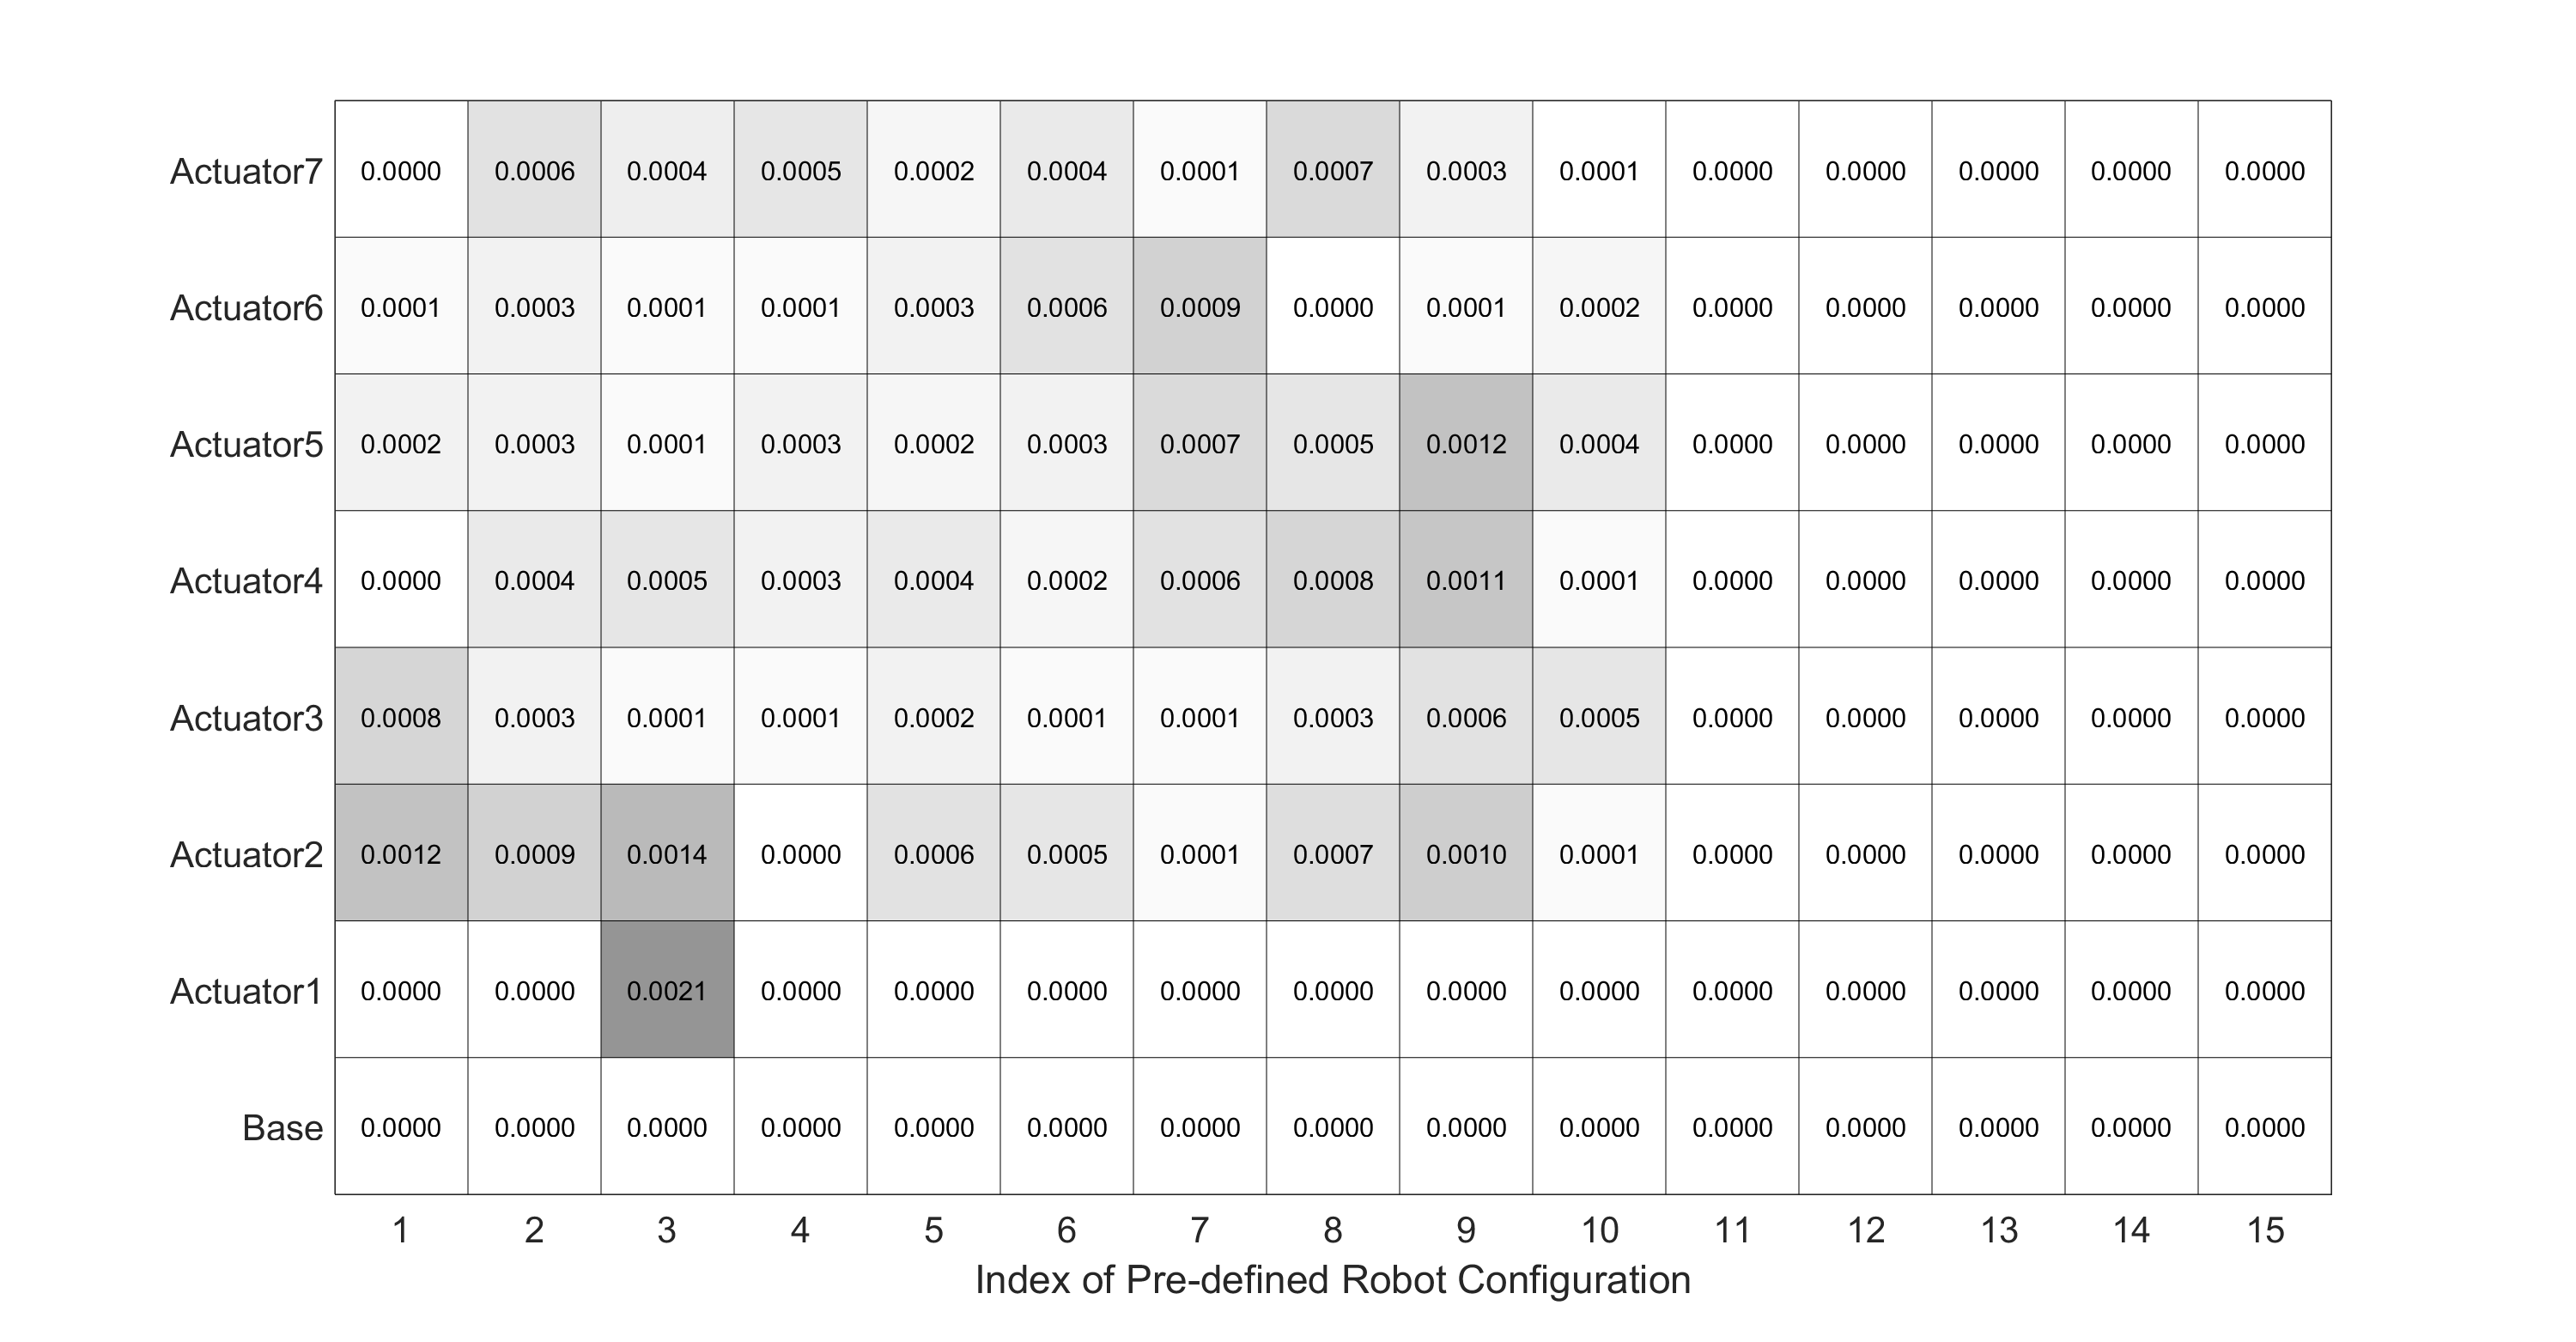
\includegraphics[width=0.9\textwidth]{./images/ForceXError.png}%
		\caption{Error of Force along X axis in N}
		\label{fig:ForceXError}%
	\end{center}
\end{figure}

\begin{figure}[H]
	\begin{center}
		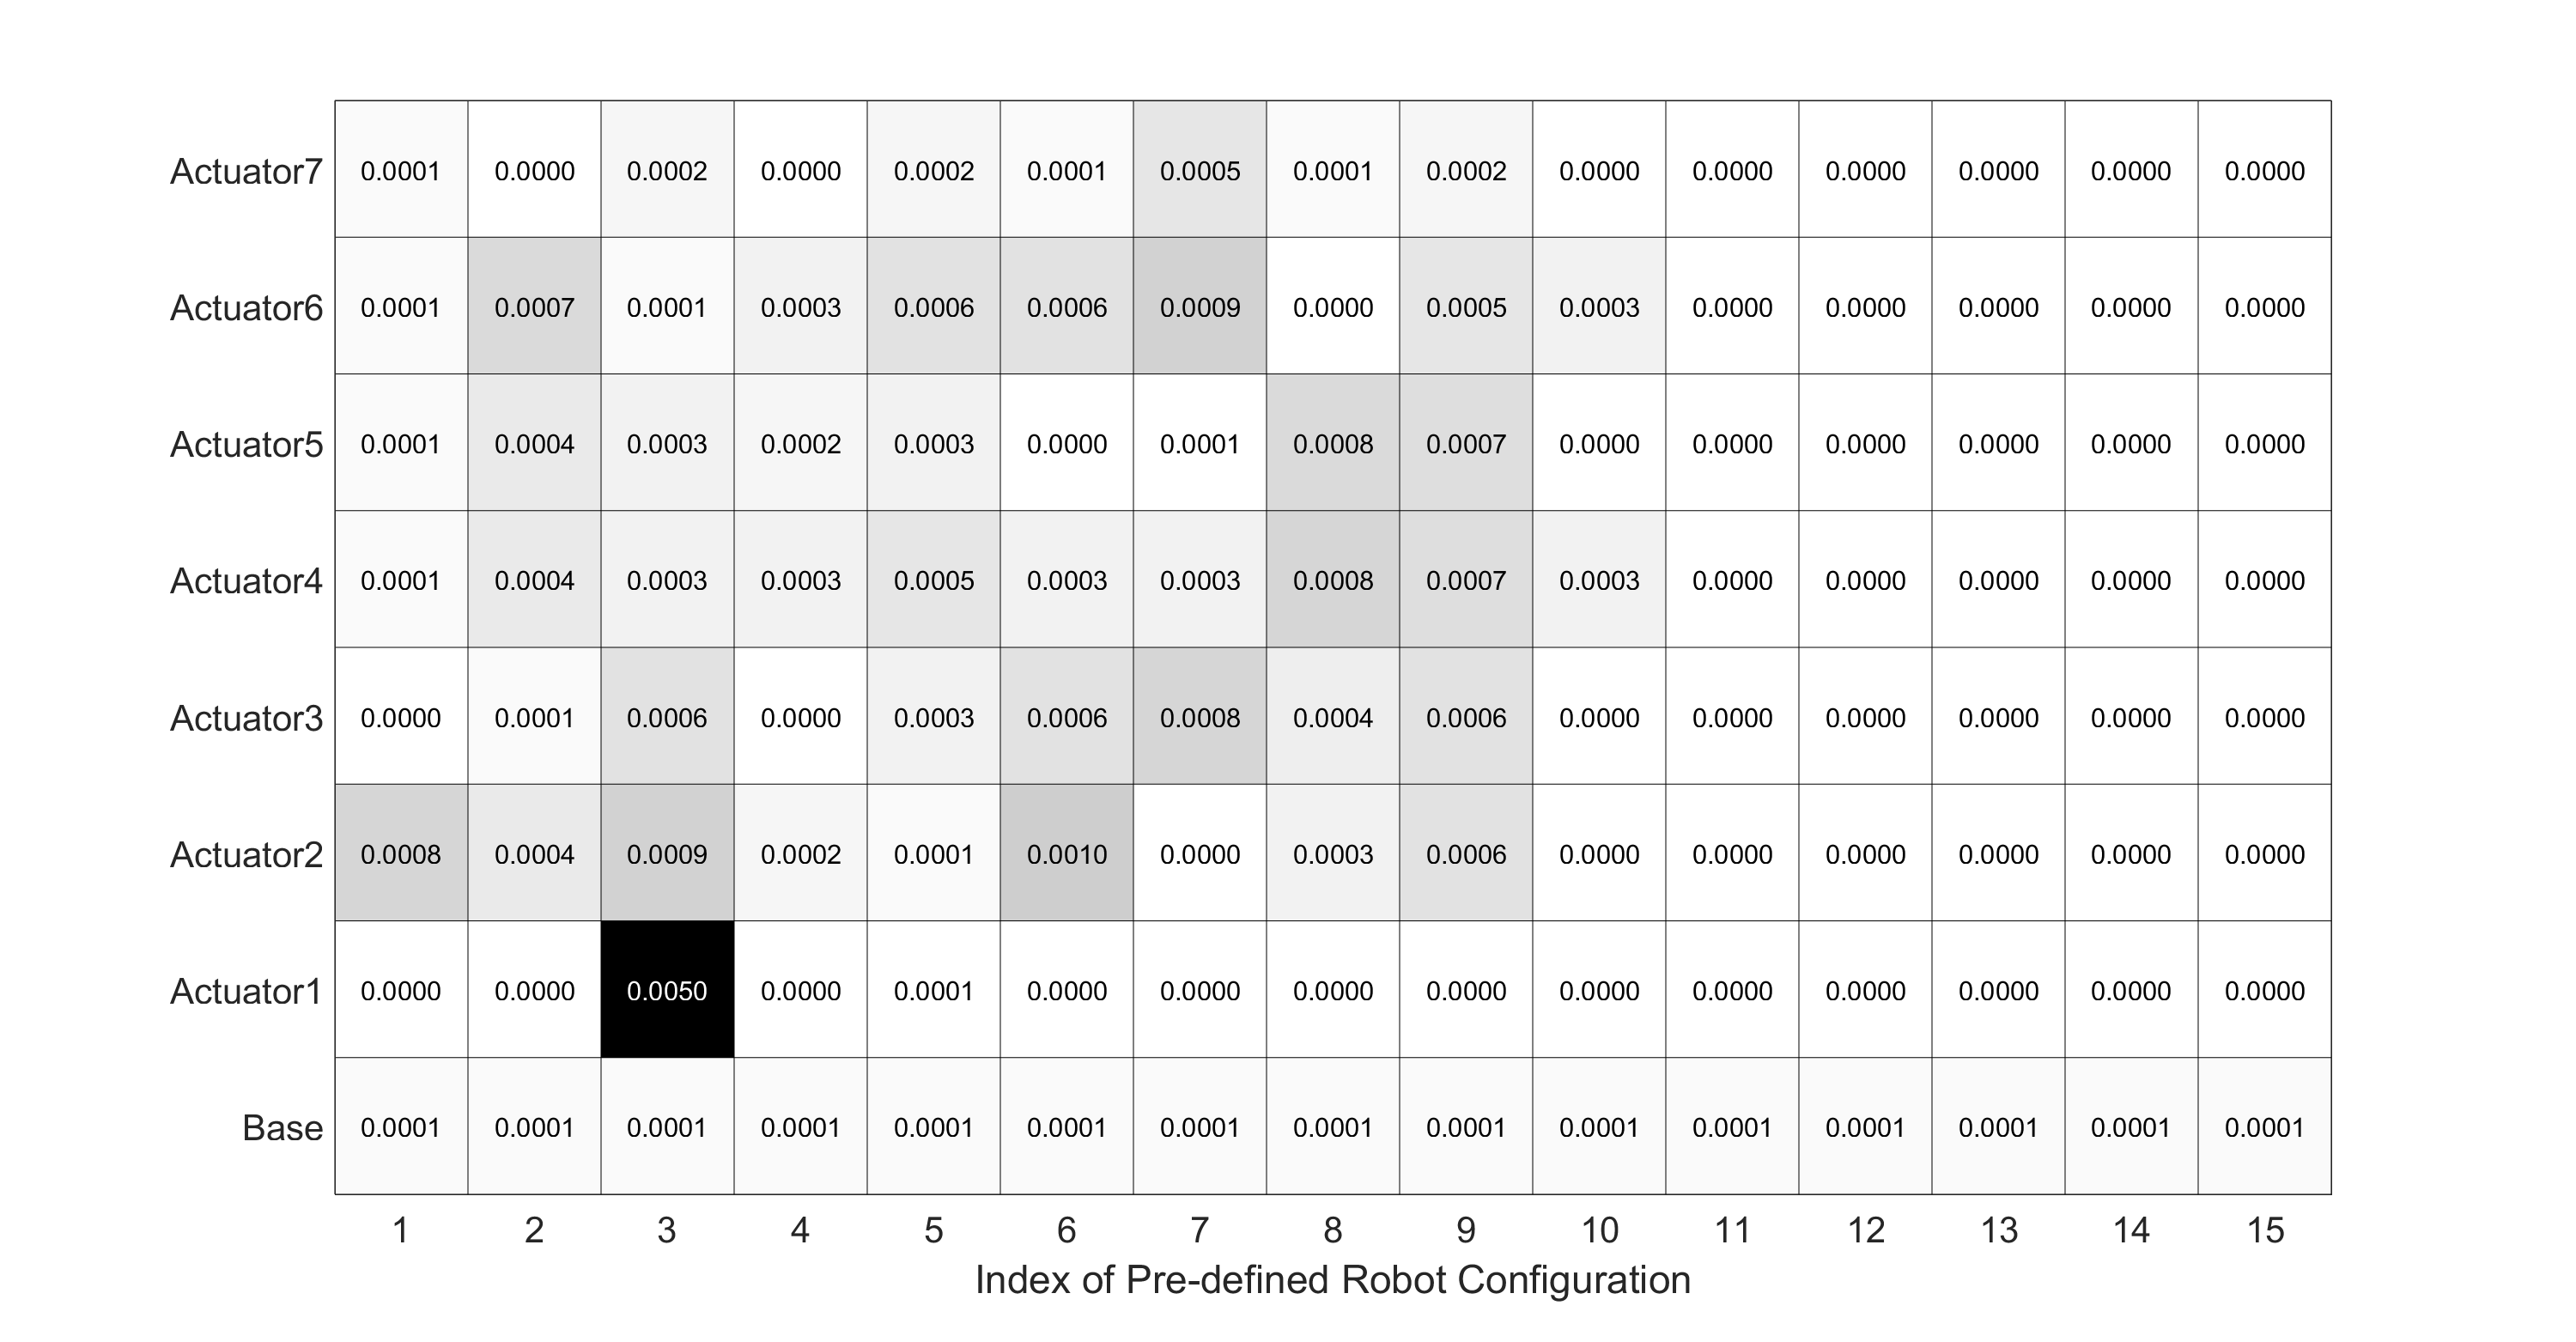
\includegraphics[width=0.9\textwidth]{./images/ForceYError.png}%
		\caption{Error of Force along Y axis in N}
		\label{fig:ForceYError}%
	\end{center}
\end{figure}

\begin{figure}[H]
	\begin{center}
		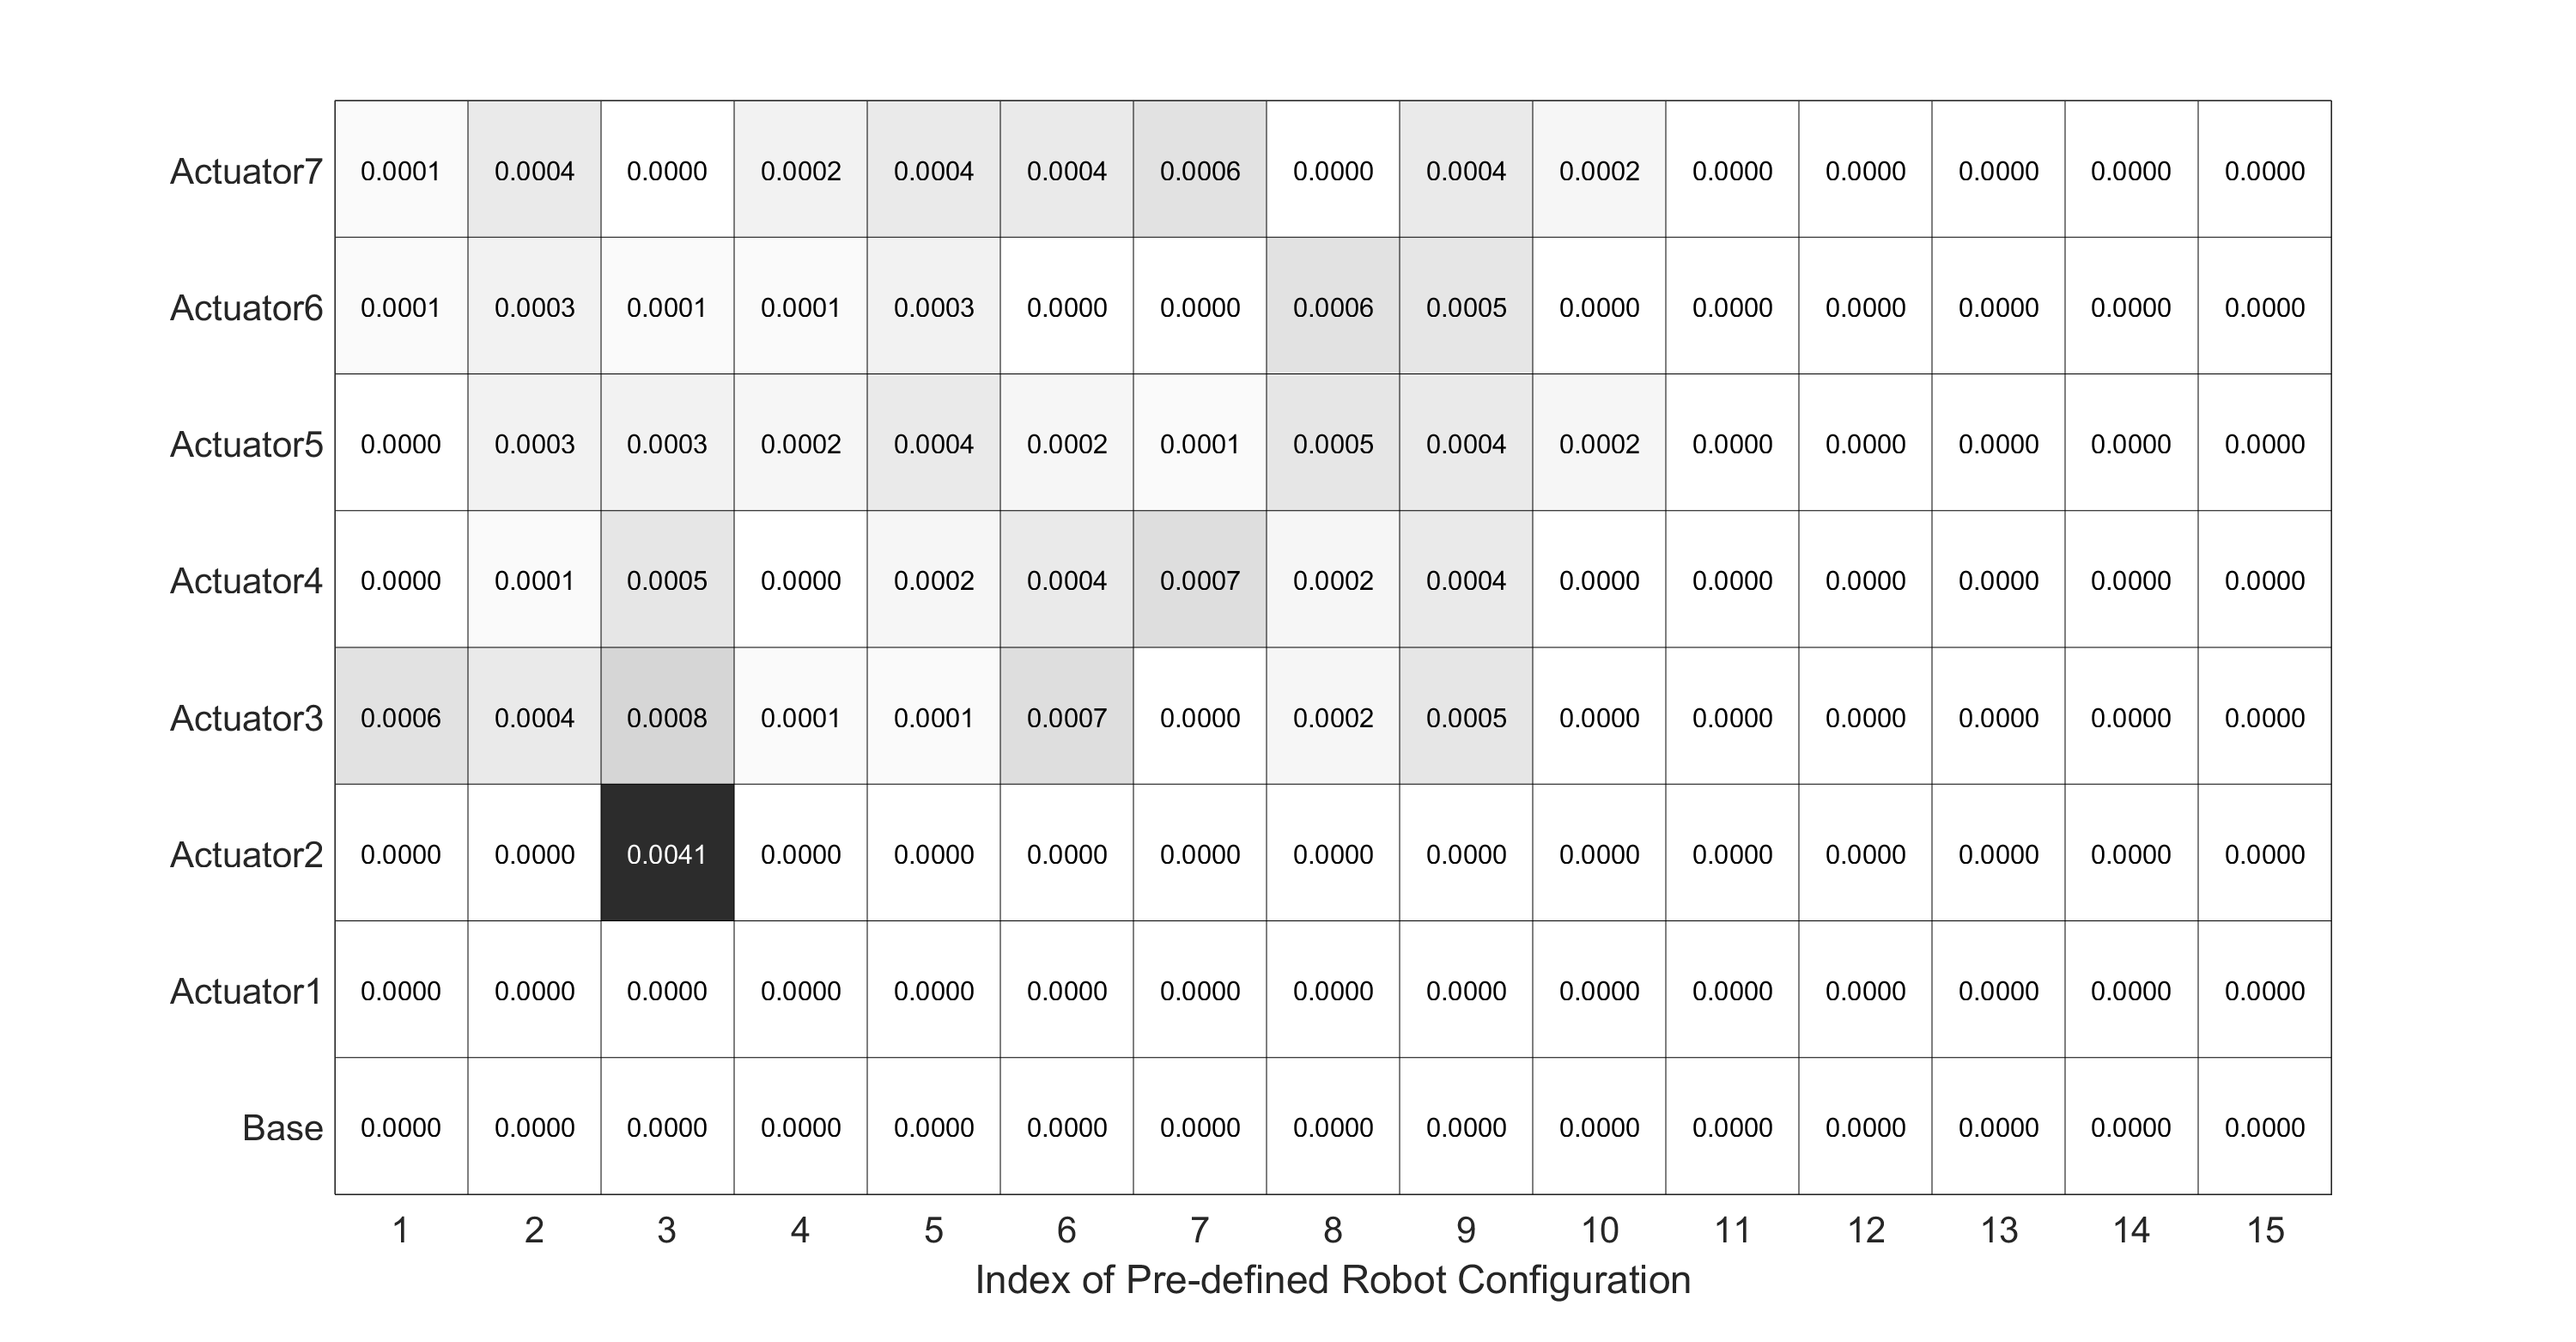
\includegraphics[width=0.9\textwidth]{./images/ForceZError.png}%
		\caption{Error of Force along Z axis in N}
		\label{fig:ForceZError}%
	\end{center}
\end{figure}

\begin{figure}[H]
	\begin{center}
		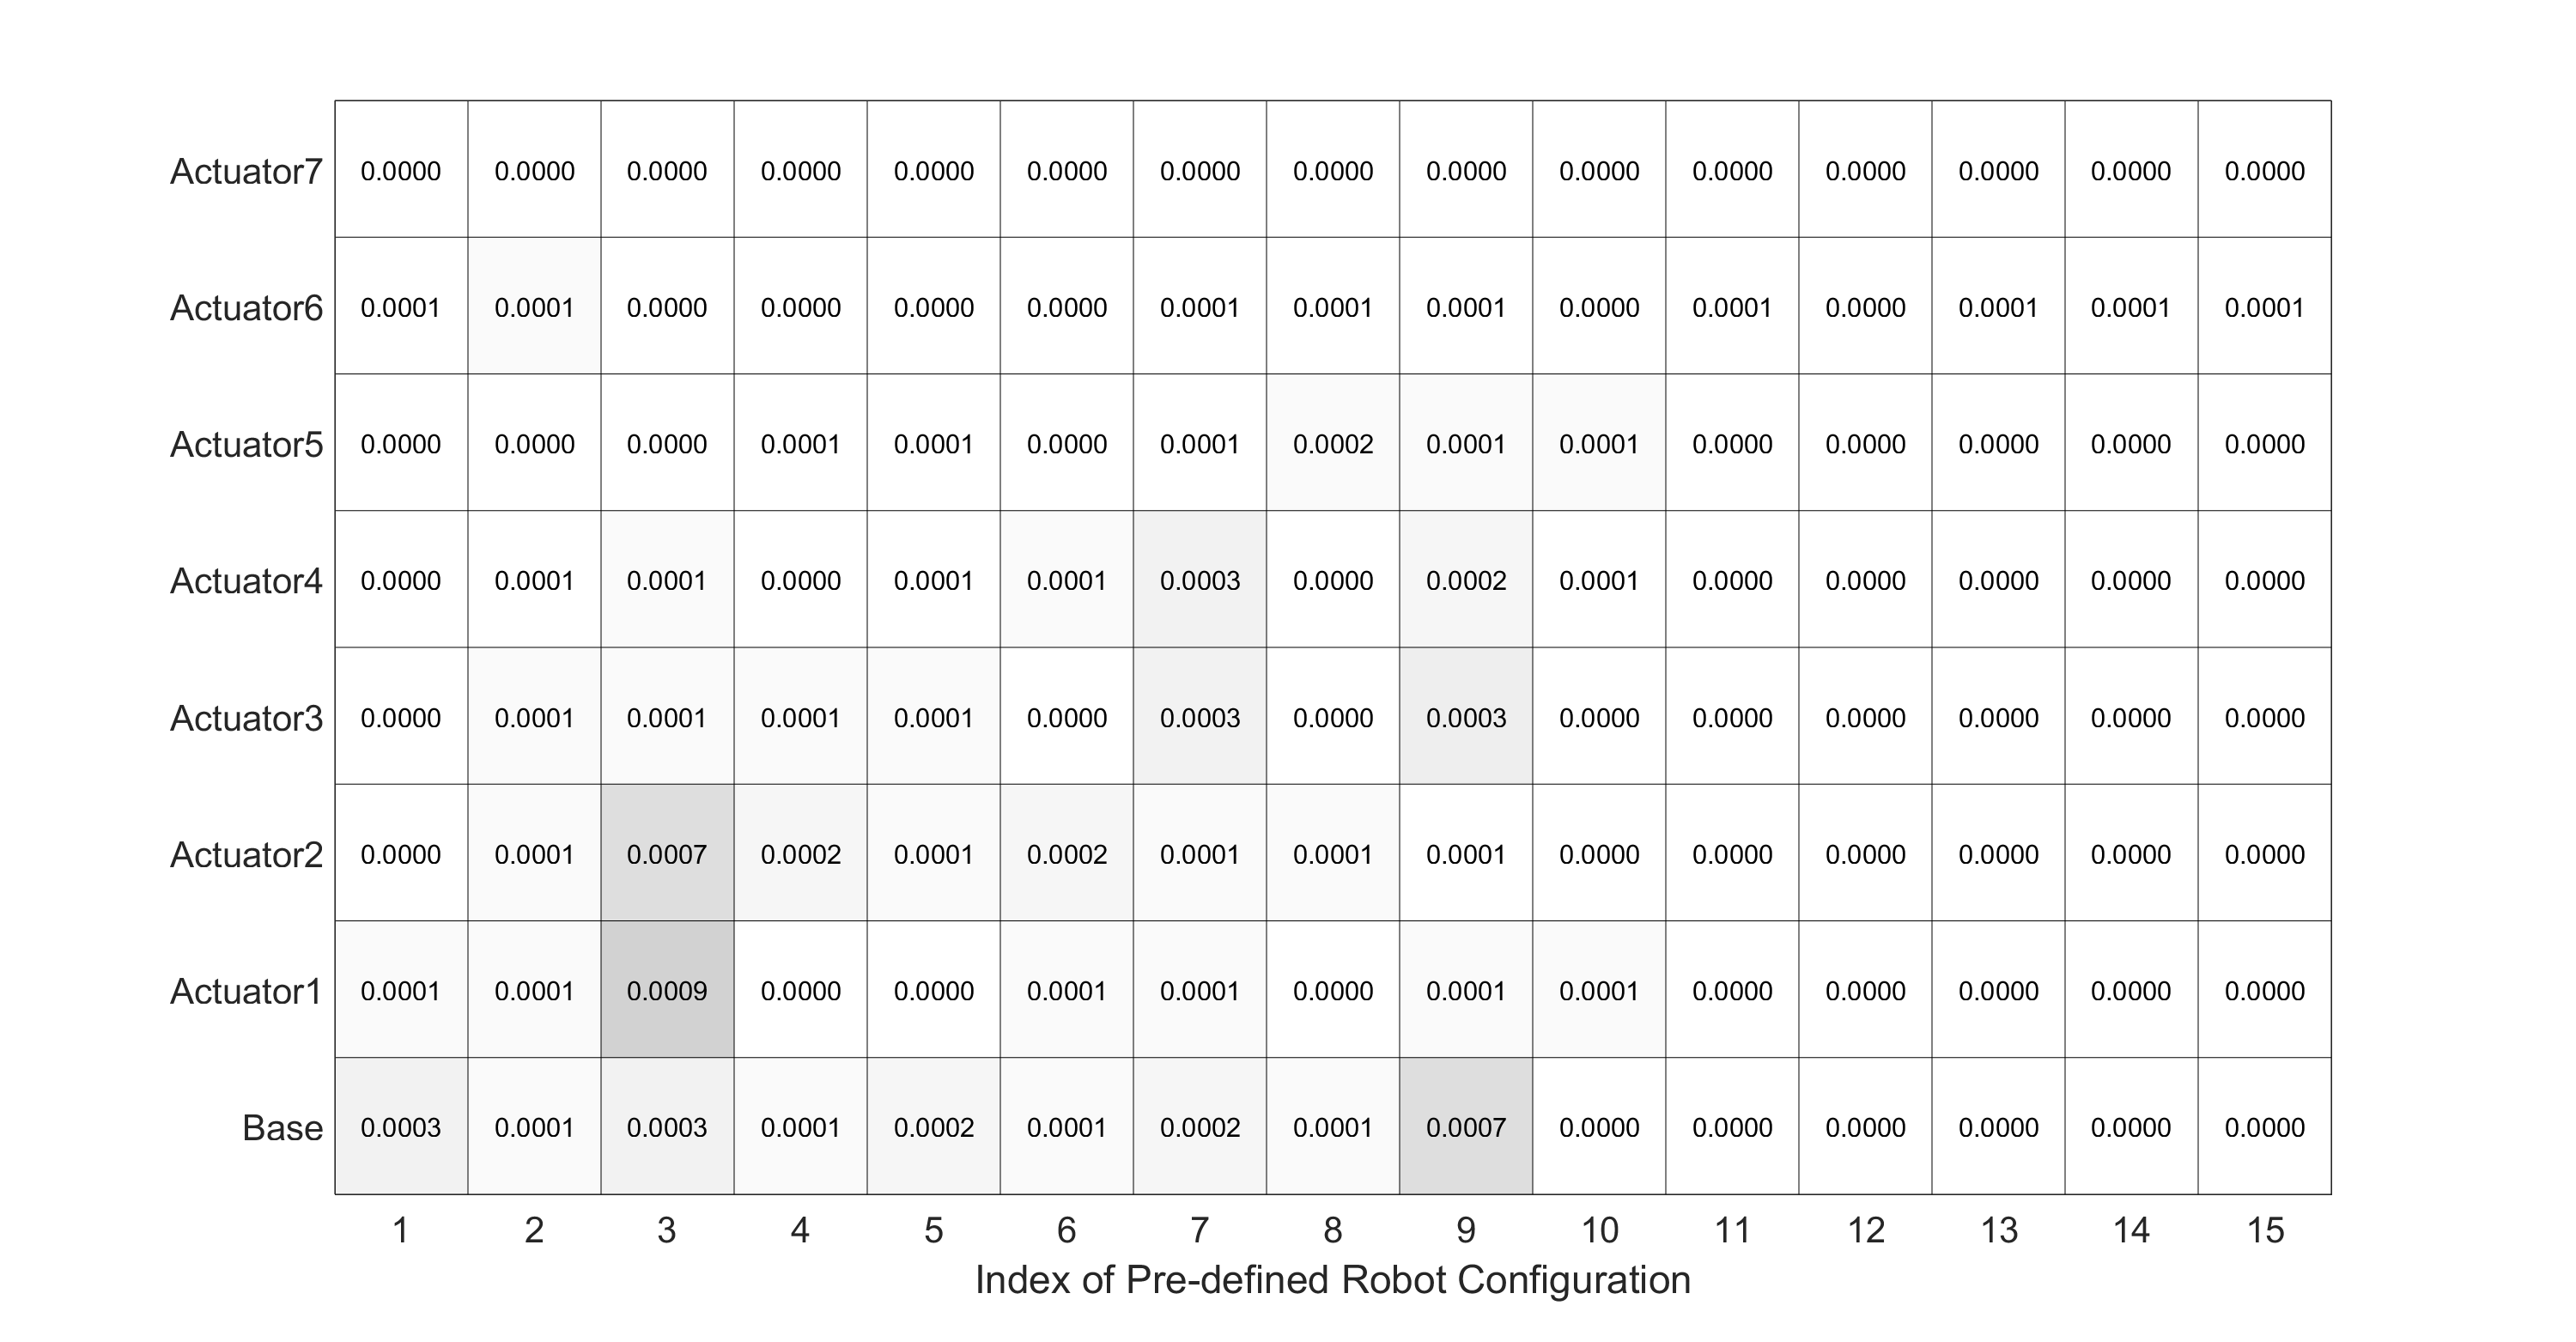
\includegraphics[width=0.9\textwidth]{./images/TorqueXError.png}%
		\caption{Error of Torque along X axis in Nm}
		\label{fig:TorqueXError}%
	\end{center}
\end{figure}

\begin{figure}[H]
	\begin{center}
		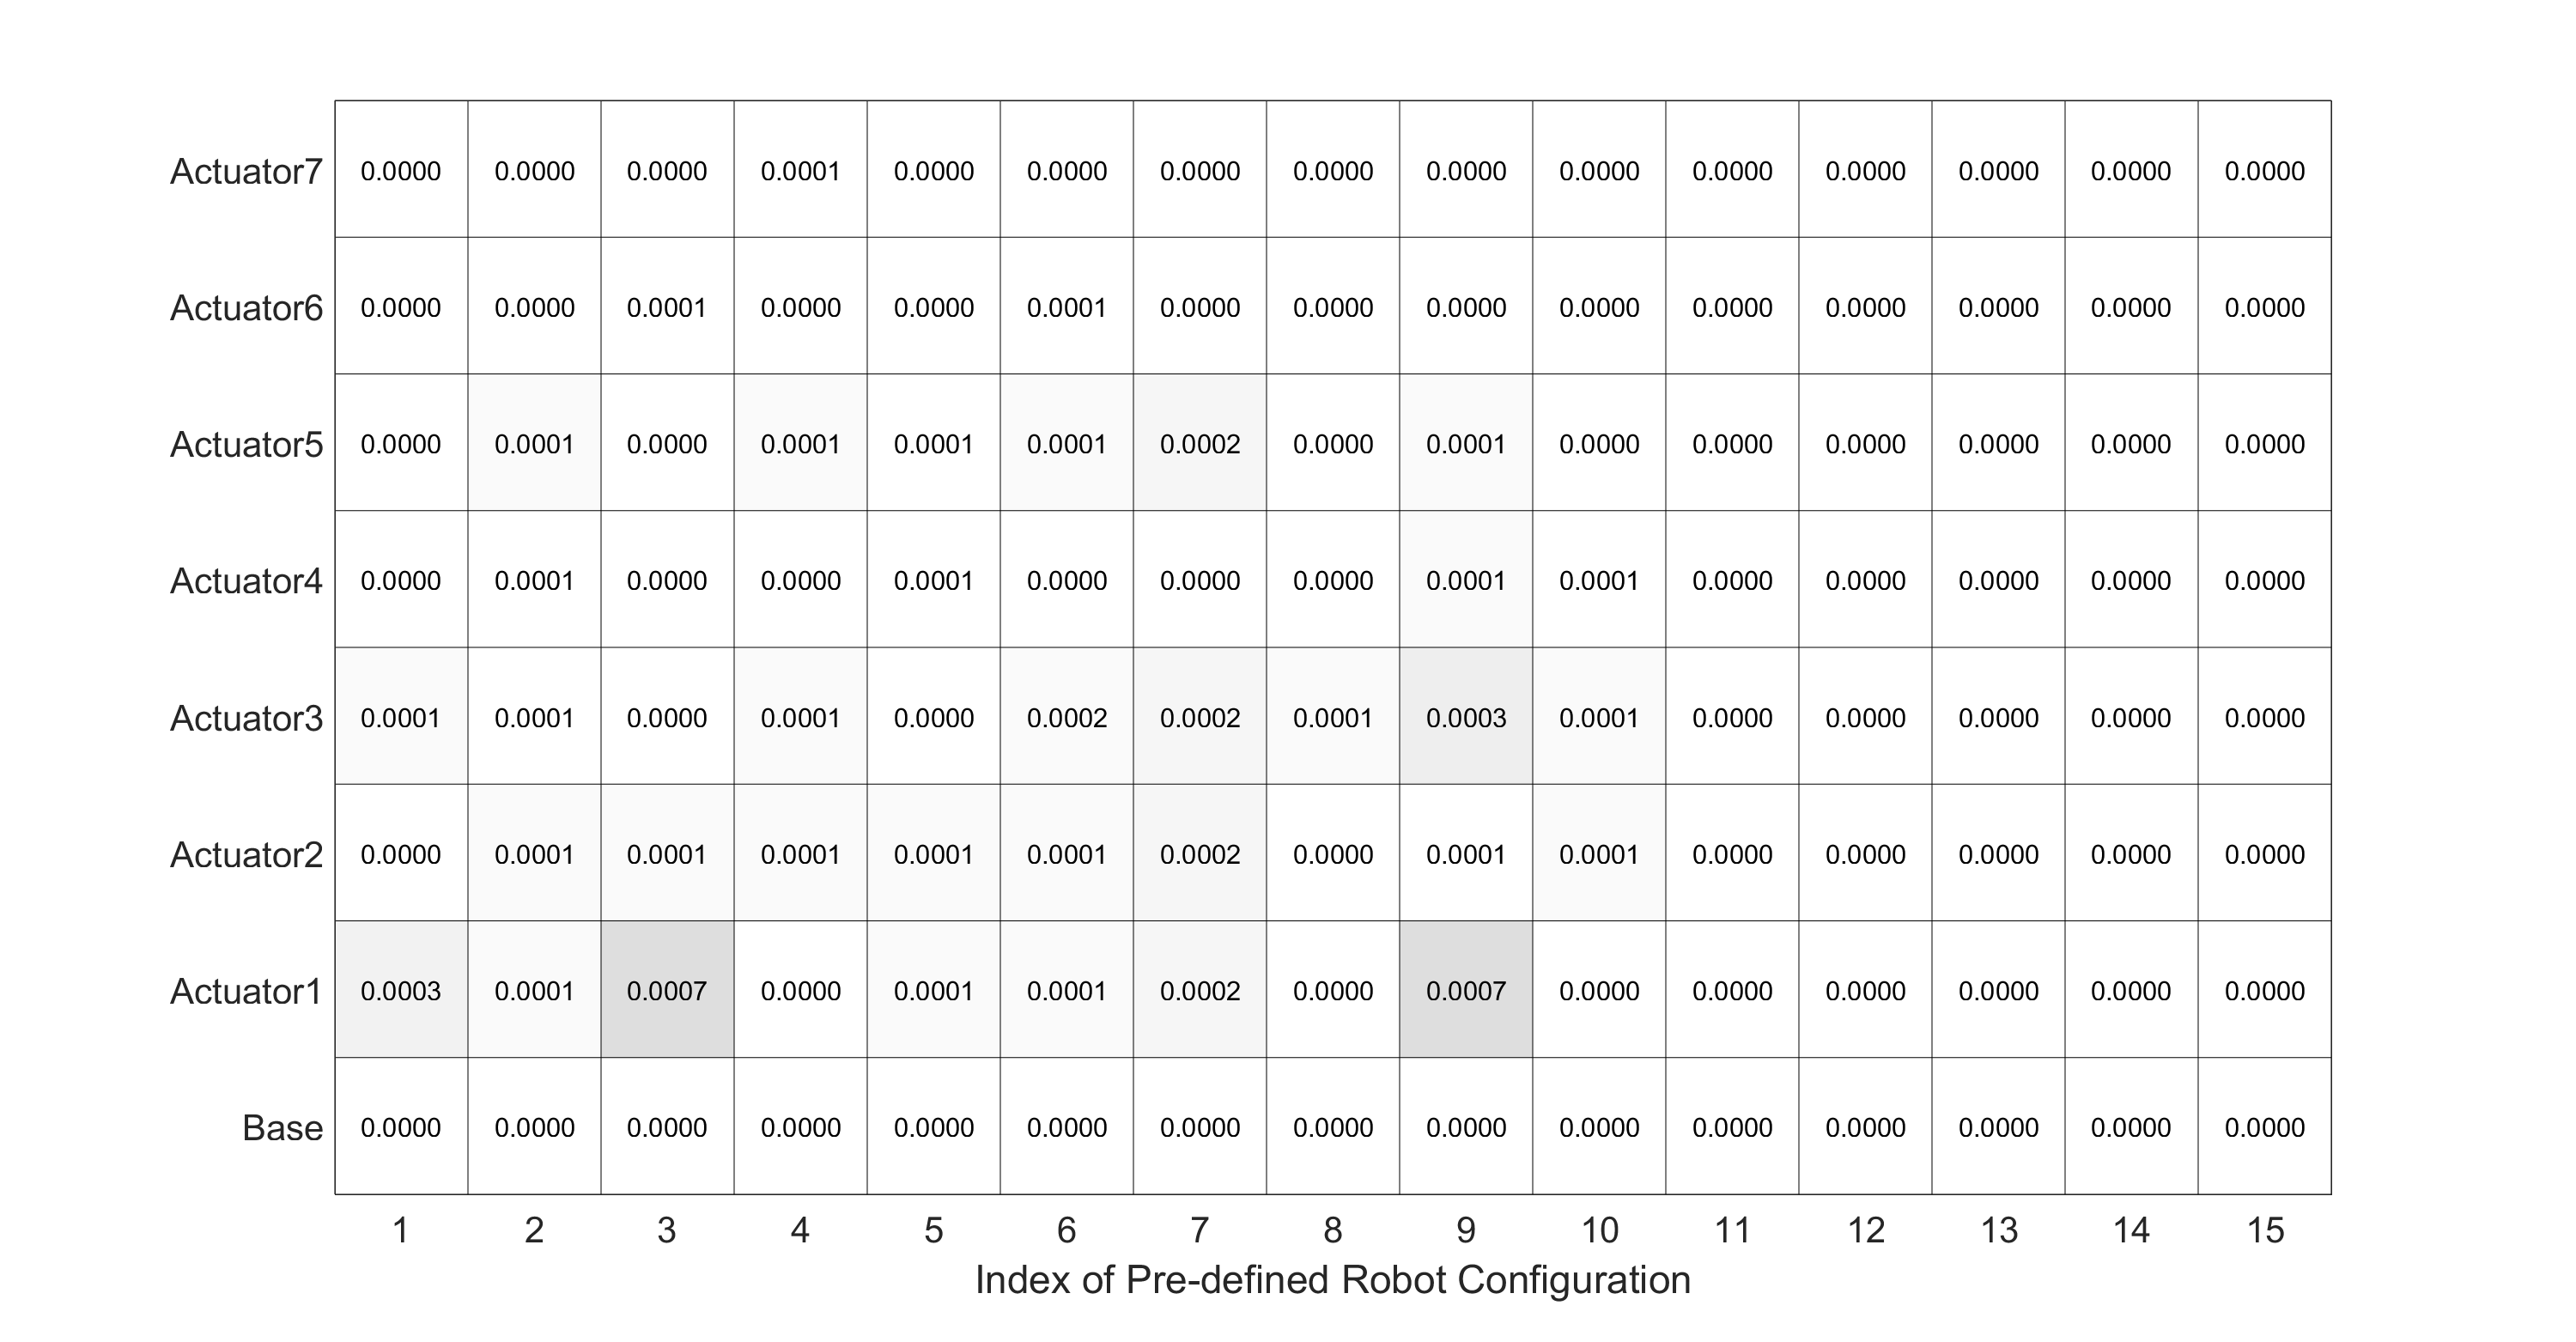
\includegraphics[width=0.9\textwidth]{./images/TorqueYError.png}%
		\caption{Error of Torque along Y axis in Nm}
		\label{fig:TorqueYError}%
	\end{center}
\end{figure}

\begin{figure}[H]
	\begin{center}
		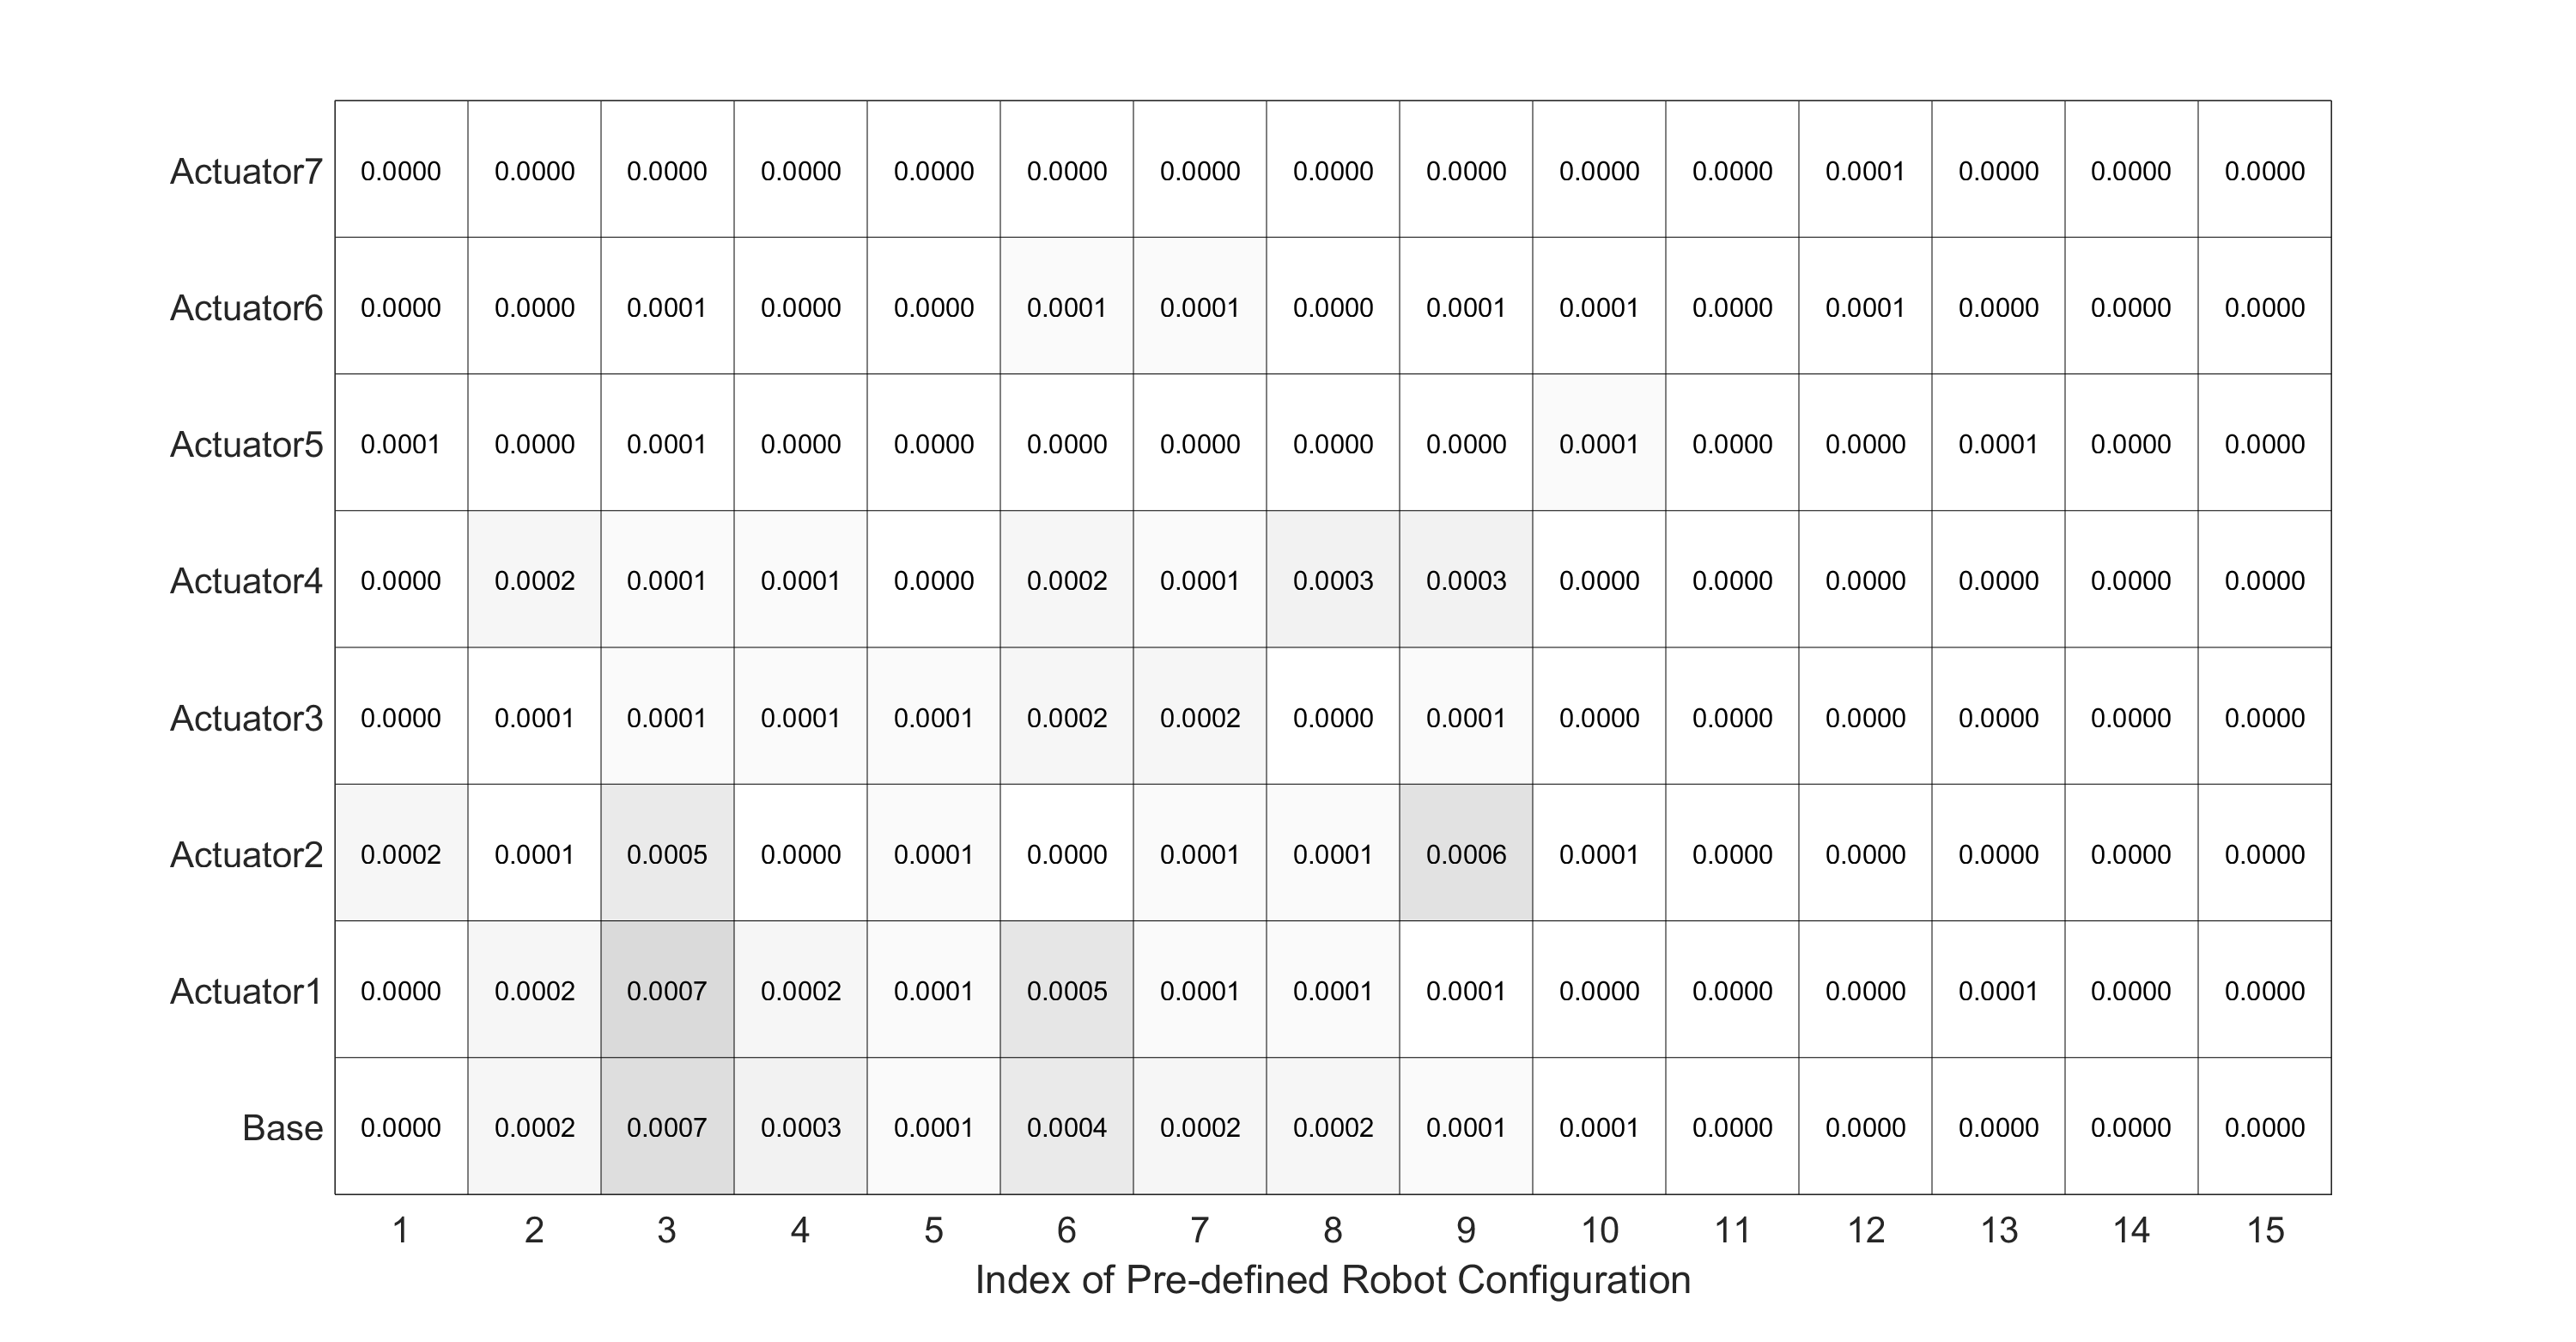
\includegraphics[width=0.9\textwidth]{./images/TorqueZError.png}%
		\caption{Error of Torque along Z axis in Nm}
		\label{fig:TorqueZError}%
	\end{center}
\end{figure}

The Figure \ref{fig:ForceXError} to Figure \ref{fig:TorqueZError} shows the error distribution of all the tests in 15 poses (horizontal axis). The vertical axis indicates the joint index, with base with index 1 and joint 7 with index 8. The color of each cell demonstrates the error of the corresponding test (the darker, the worse). In worst cases, the error of joint force reach 0.005N and torque is around 0.001Nm. 

It is noticed that the robot cannot perfectly reach the predefined configurations. It is more meaningful to compute JointWrench\_PC based on robot joint position feedback for the comparison, as shown in Figure \ref{fig:ForceXErrorFB}to Figure \ref{fig:TorqueZErrorFB}. It is obvious that differences are ten times smaller, in the scale of $10^{-4}$ N (Force) or Nm(Torque). This difference may due to the provided data precision in the code or computation round up. 


\begin{figure}[H]
	\begin{center}
		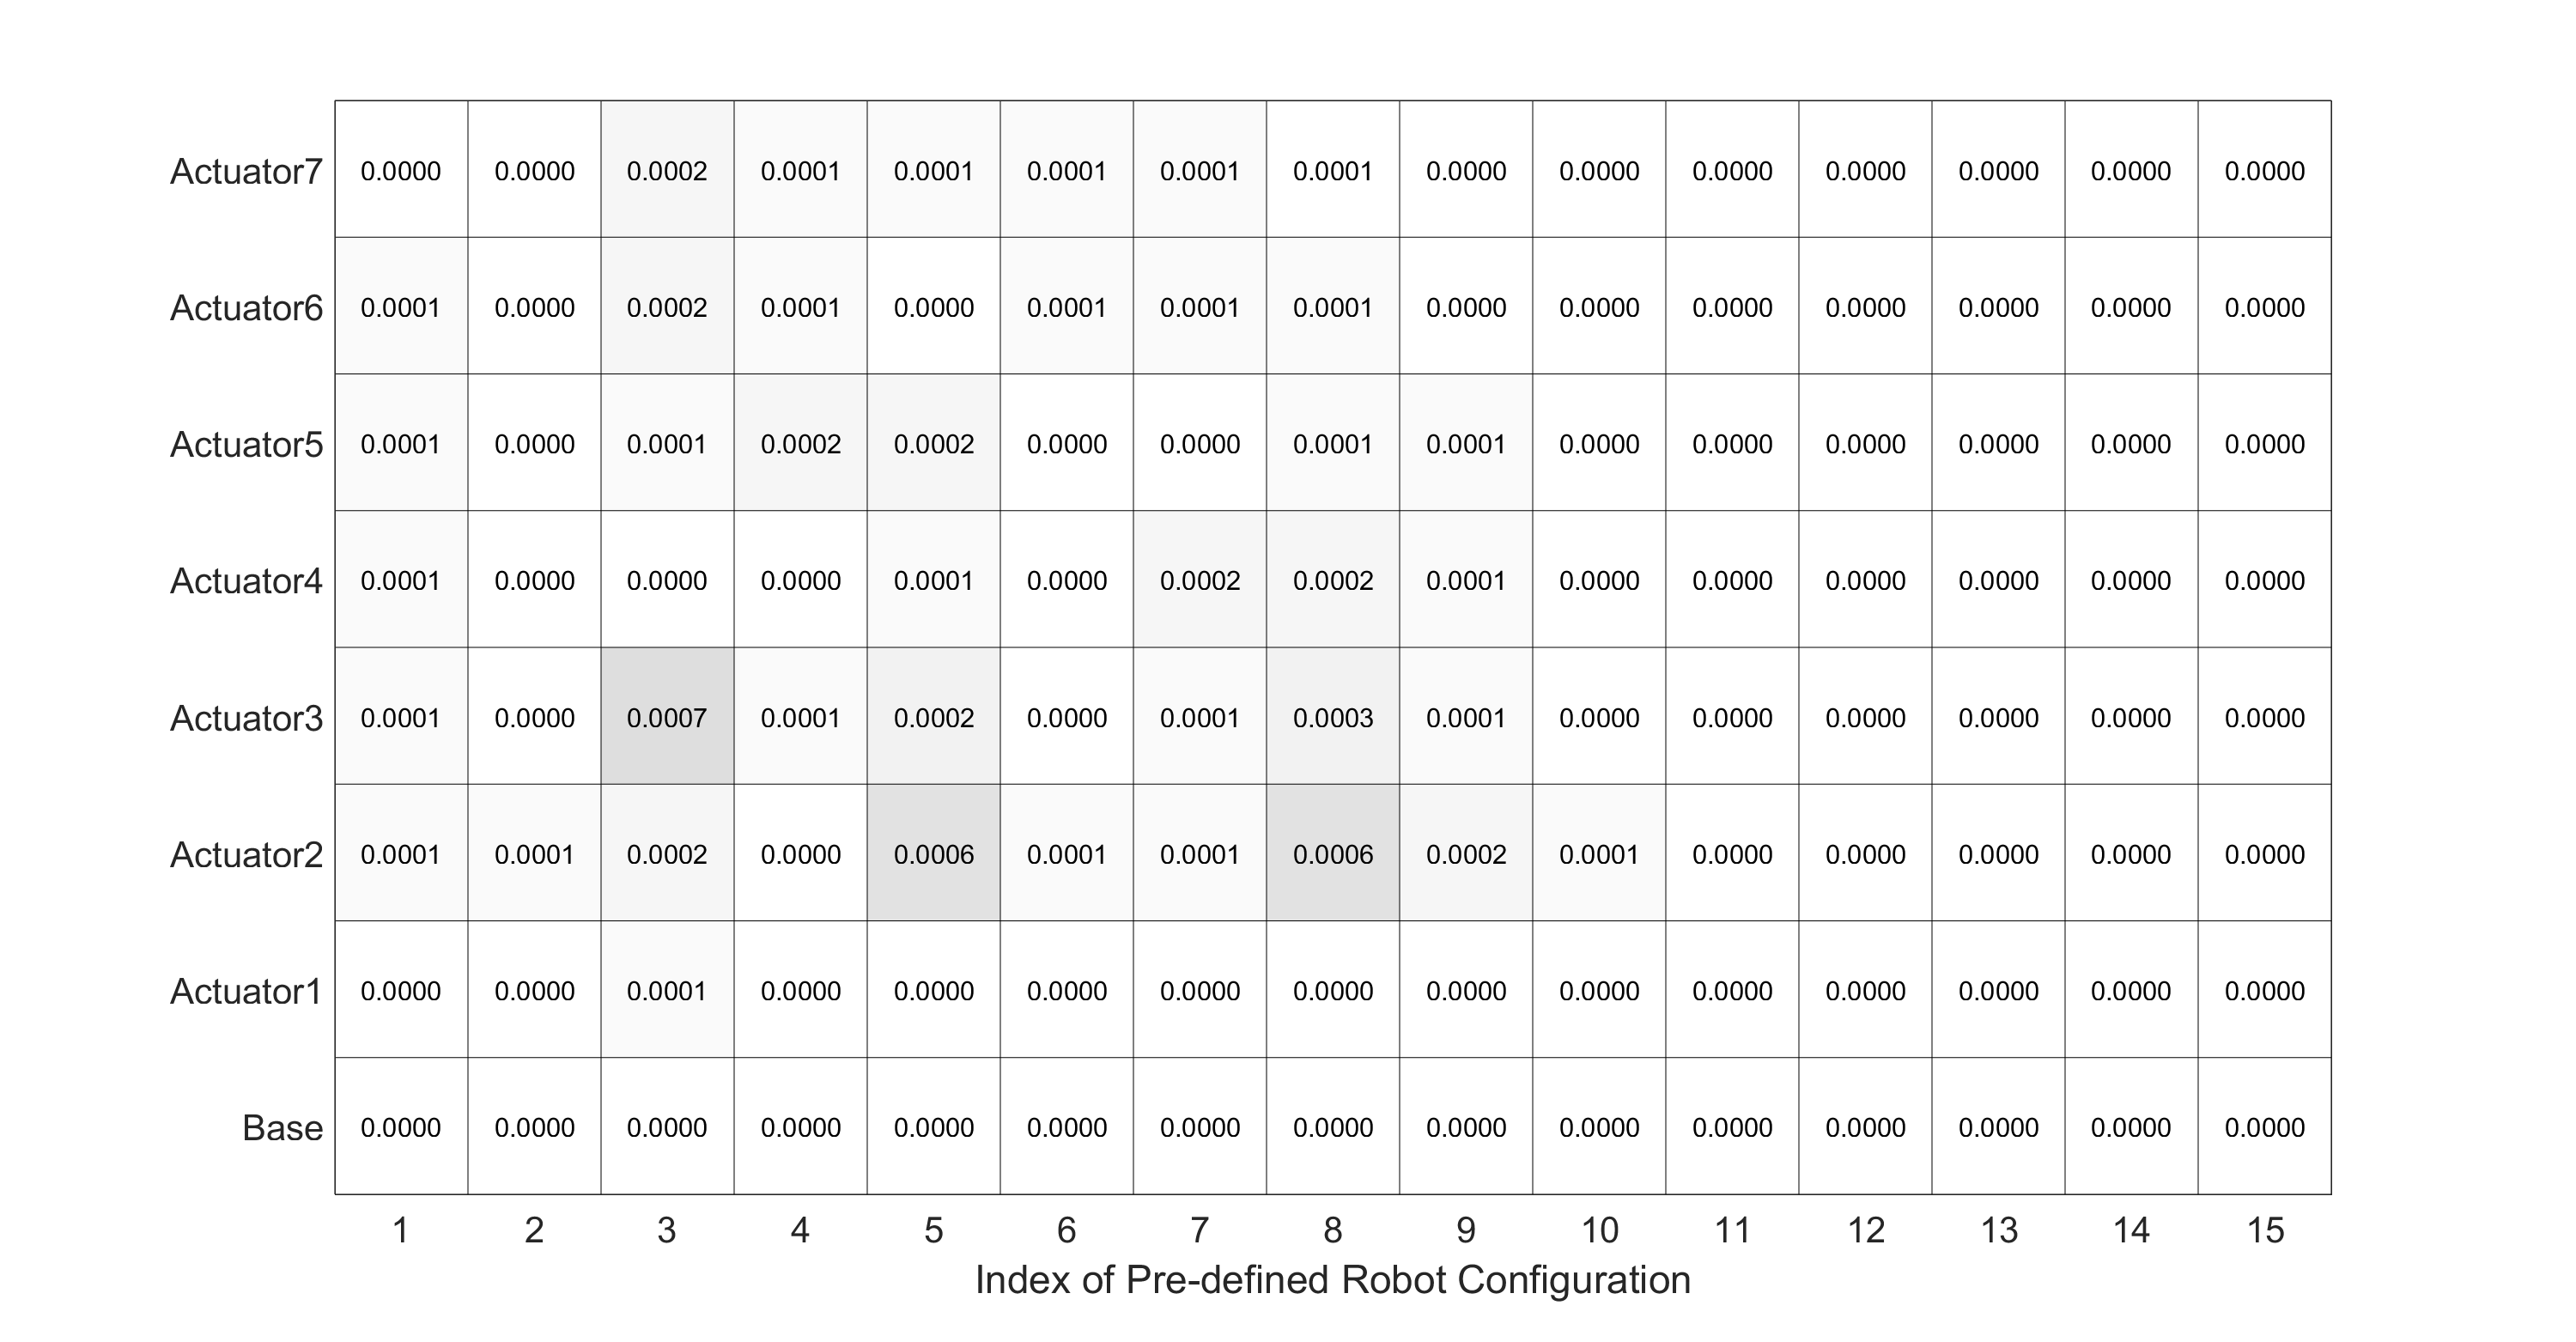
\includegraphics[width=0.9\textwidth]{./images/ForceXErrorFB.png}%
		\caption{Error of Force along X axis in N}
		\label{fig:ForceXErrorFB}%
	\end{center}
\end{figure}

\begin{figure}[H]
	\begin{center}
		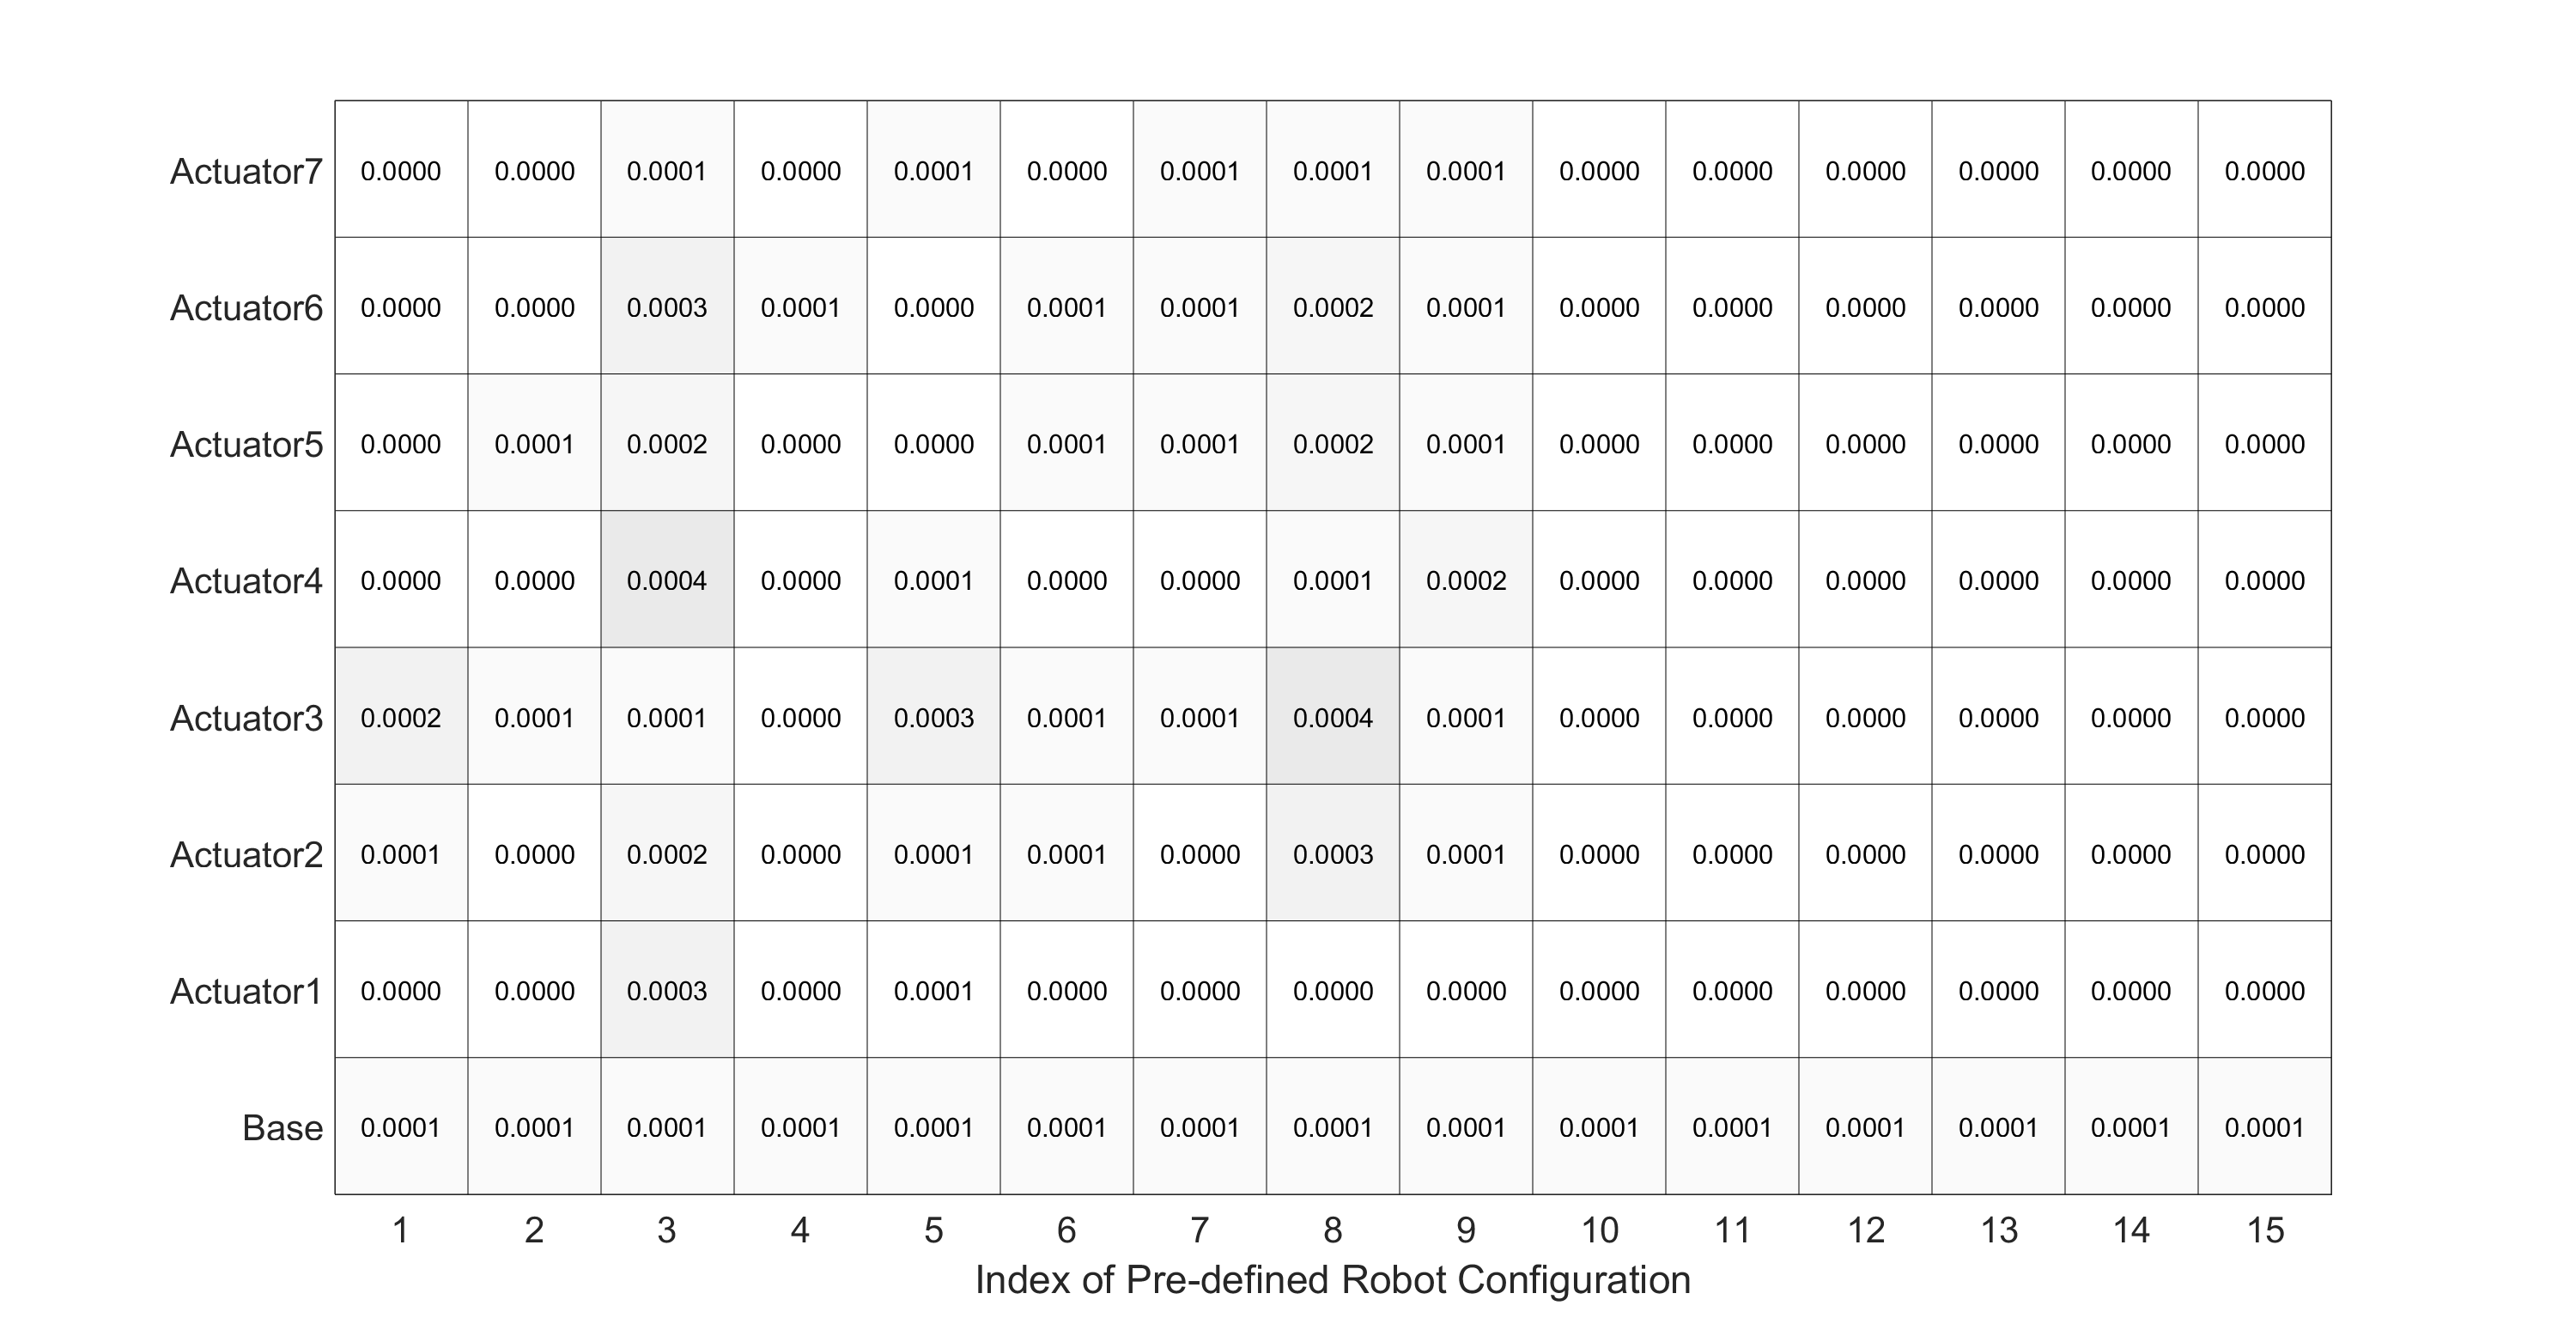
\includegraphics[width=0.9\textwidth]{./images/ForceYErrorFB.png}%
		\caption{Error of Force along Y axis in N}
		\label{fig:ForceYErrorFB}%
	\end{center}
\end{figure}

\begin{figure}[H]
	\begin{center}
		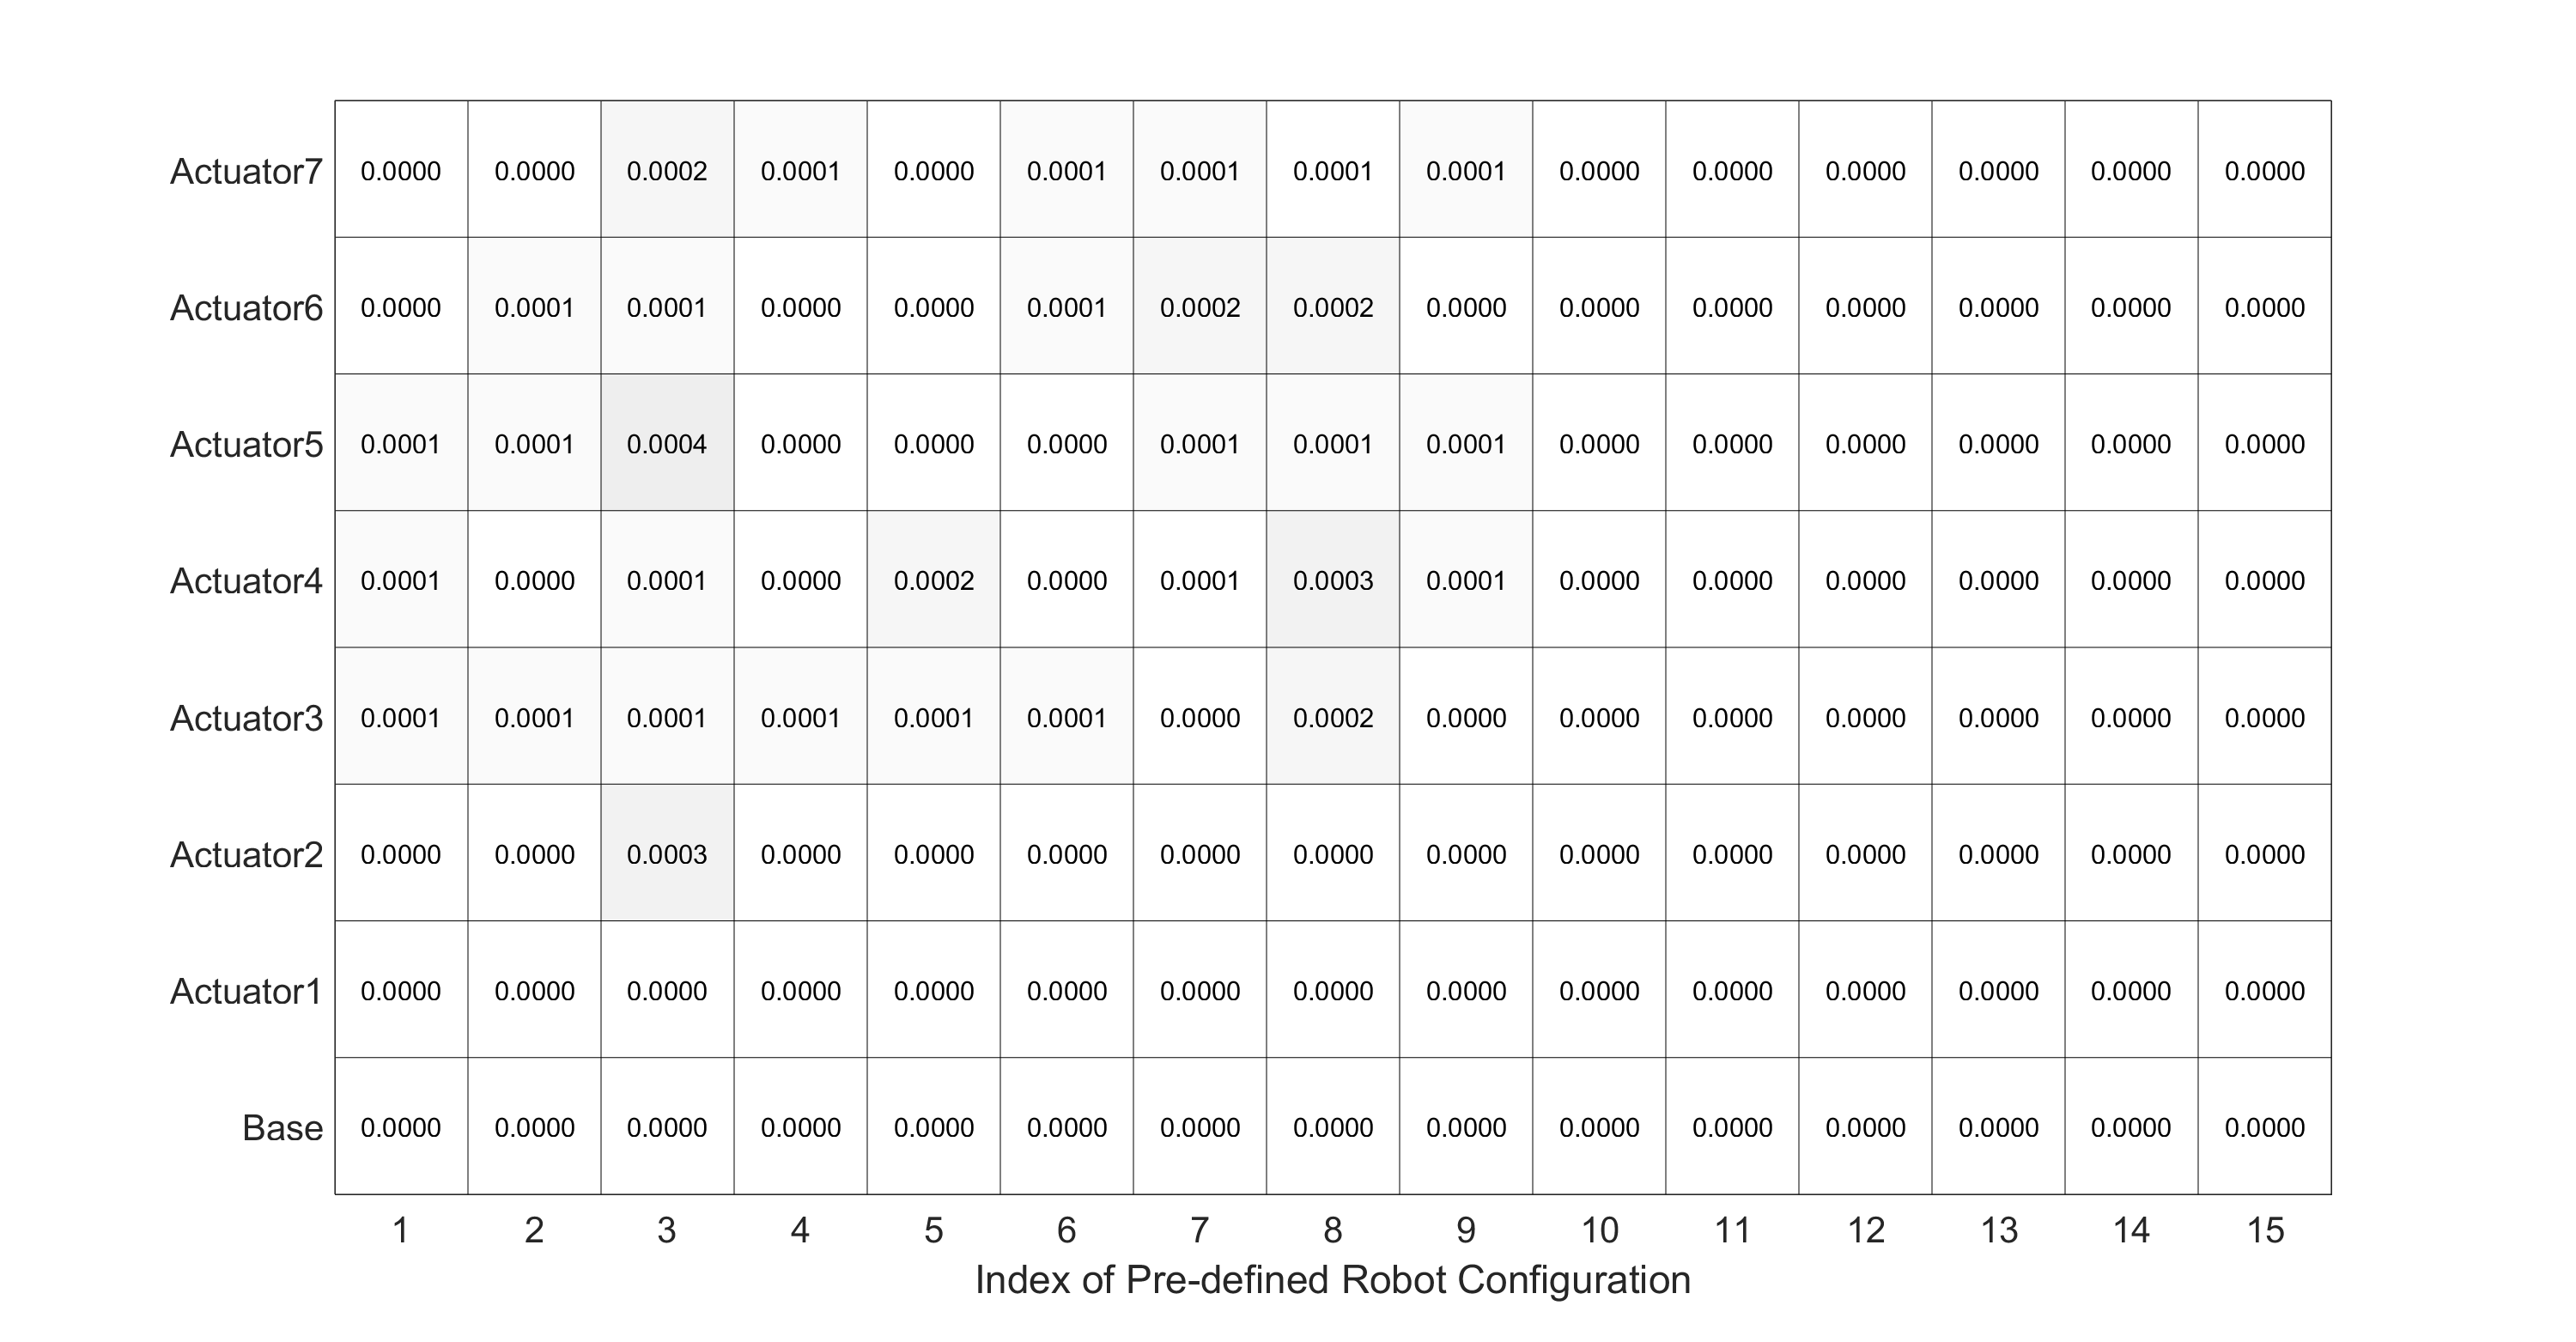
\includegraphics[width=0.9\textwidth]{./images/ForceZErrorFB.png}%
		\caption{Error of Force along Z axis in N}
		\label{fig:ForceZErrorFB}%
	\end{center}
\end{figure}

\begin{figure}[H]
	\begin{center}
		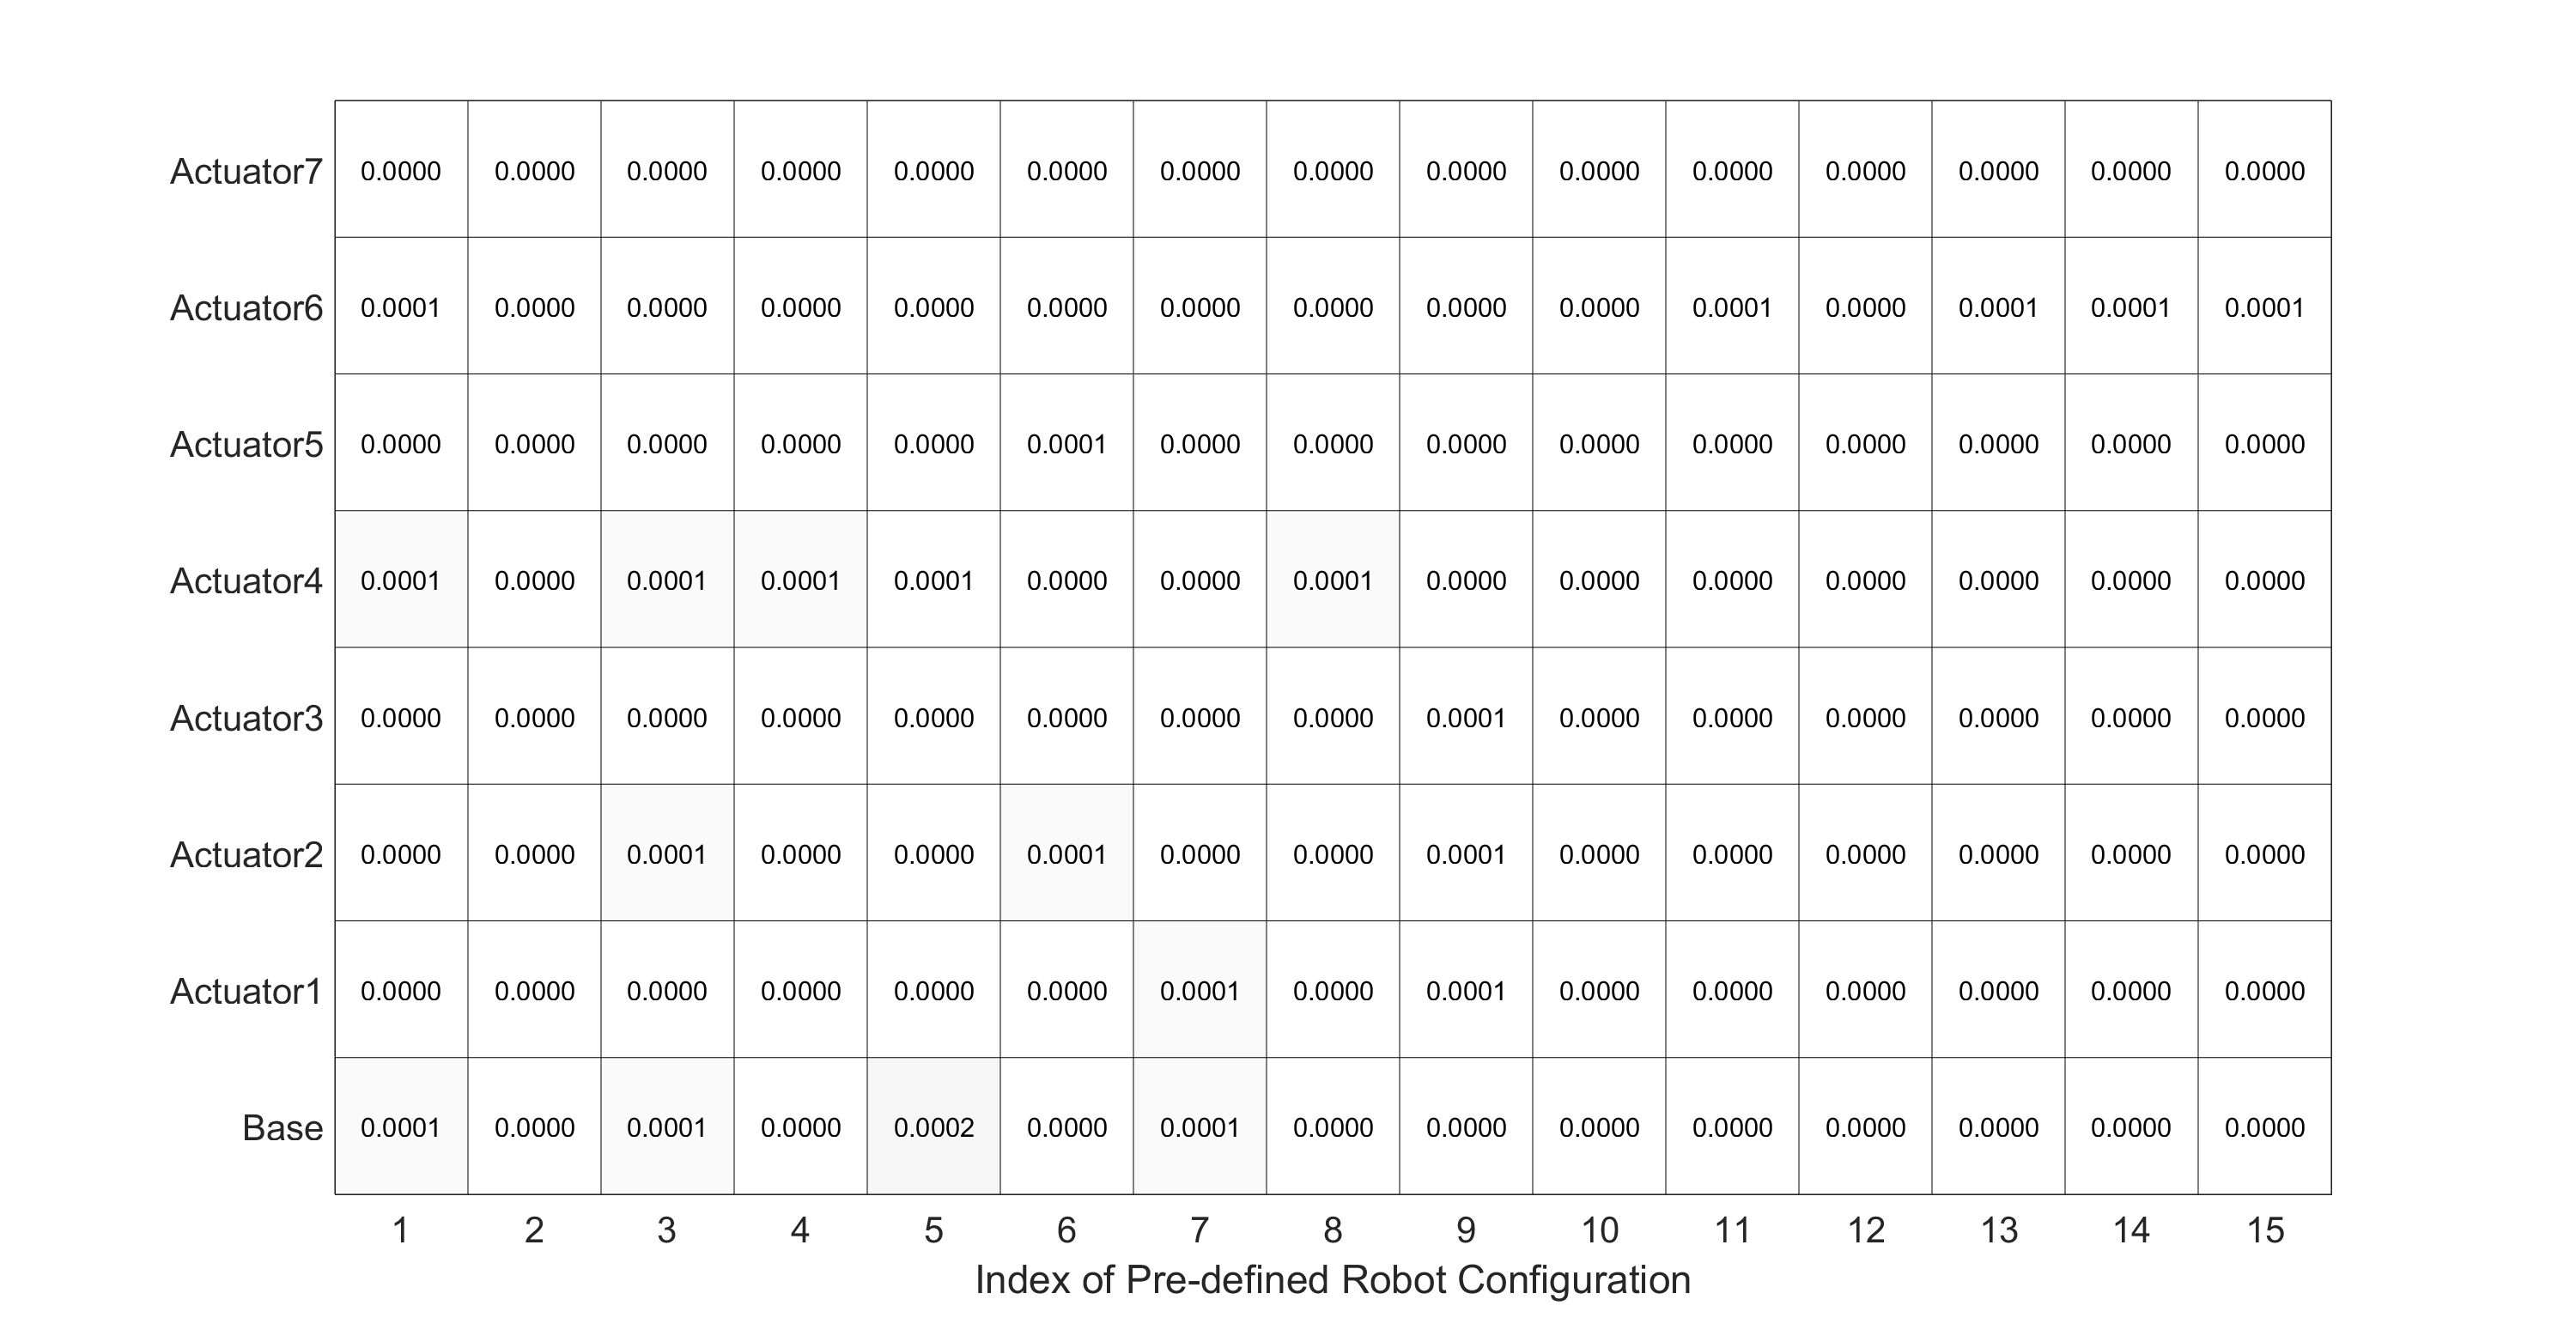
\includegraphics[width=0.9\textwidth]{./images/TorqueXErrorFB.png}%
		\caption{Error of Torque along X axis in Nm}
		\label{fig:TorqueXErrorFB}%
	\end{center}
\end{figure}

\begin{figure}[H]
	\begin{center}
		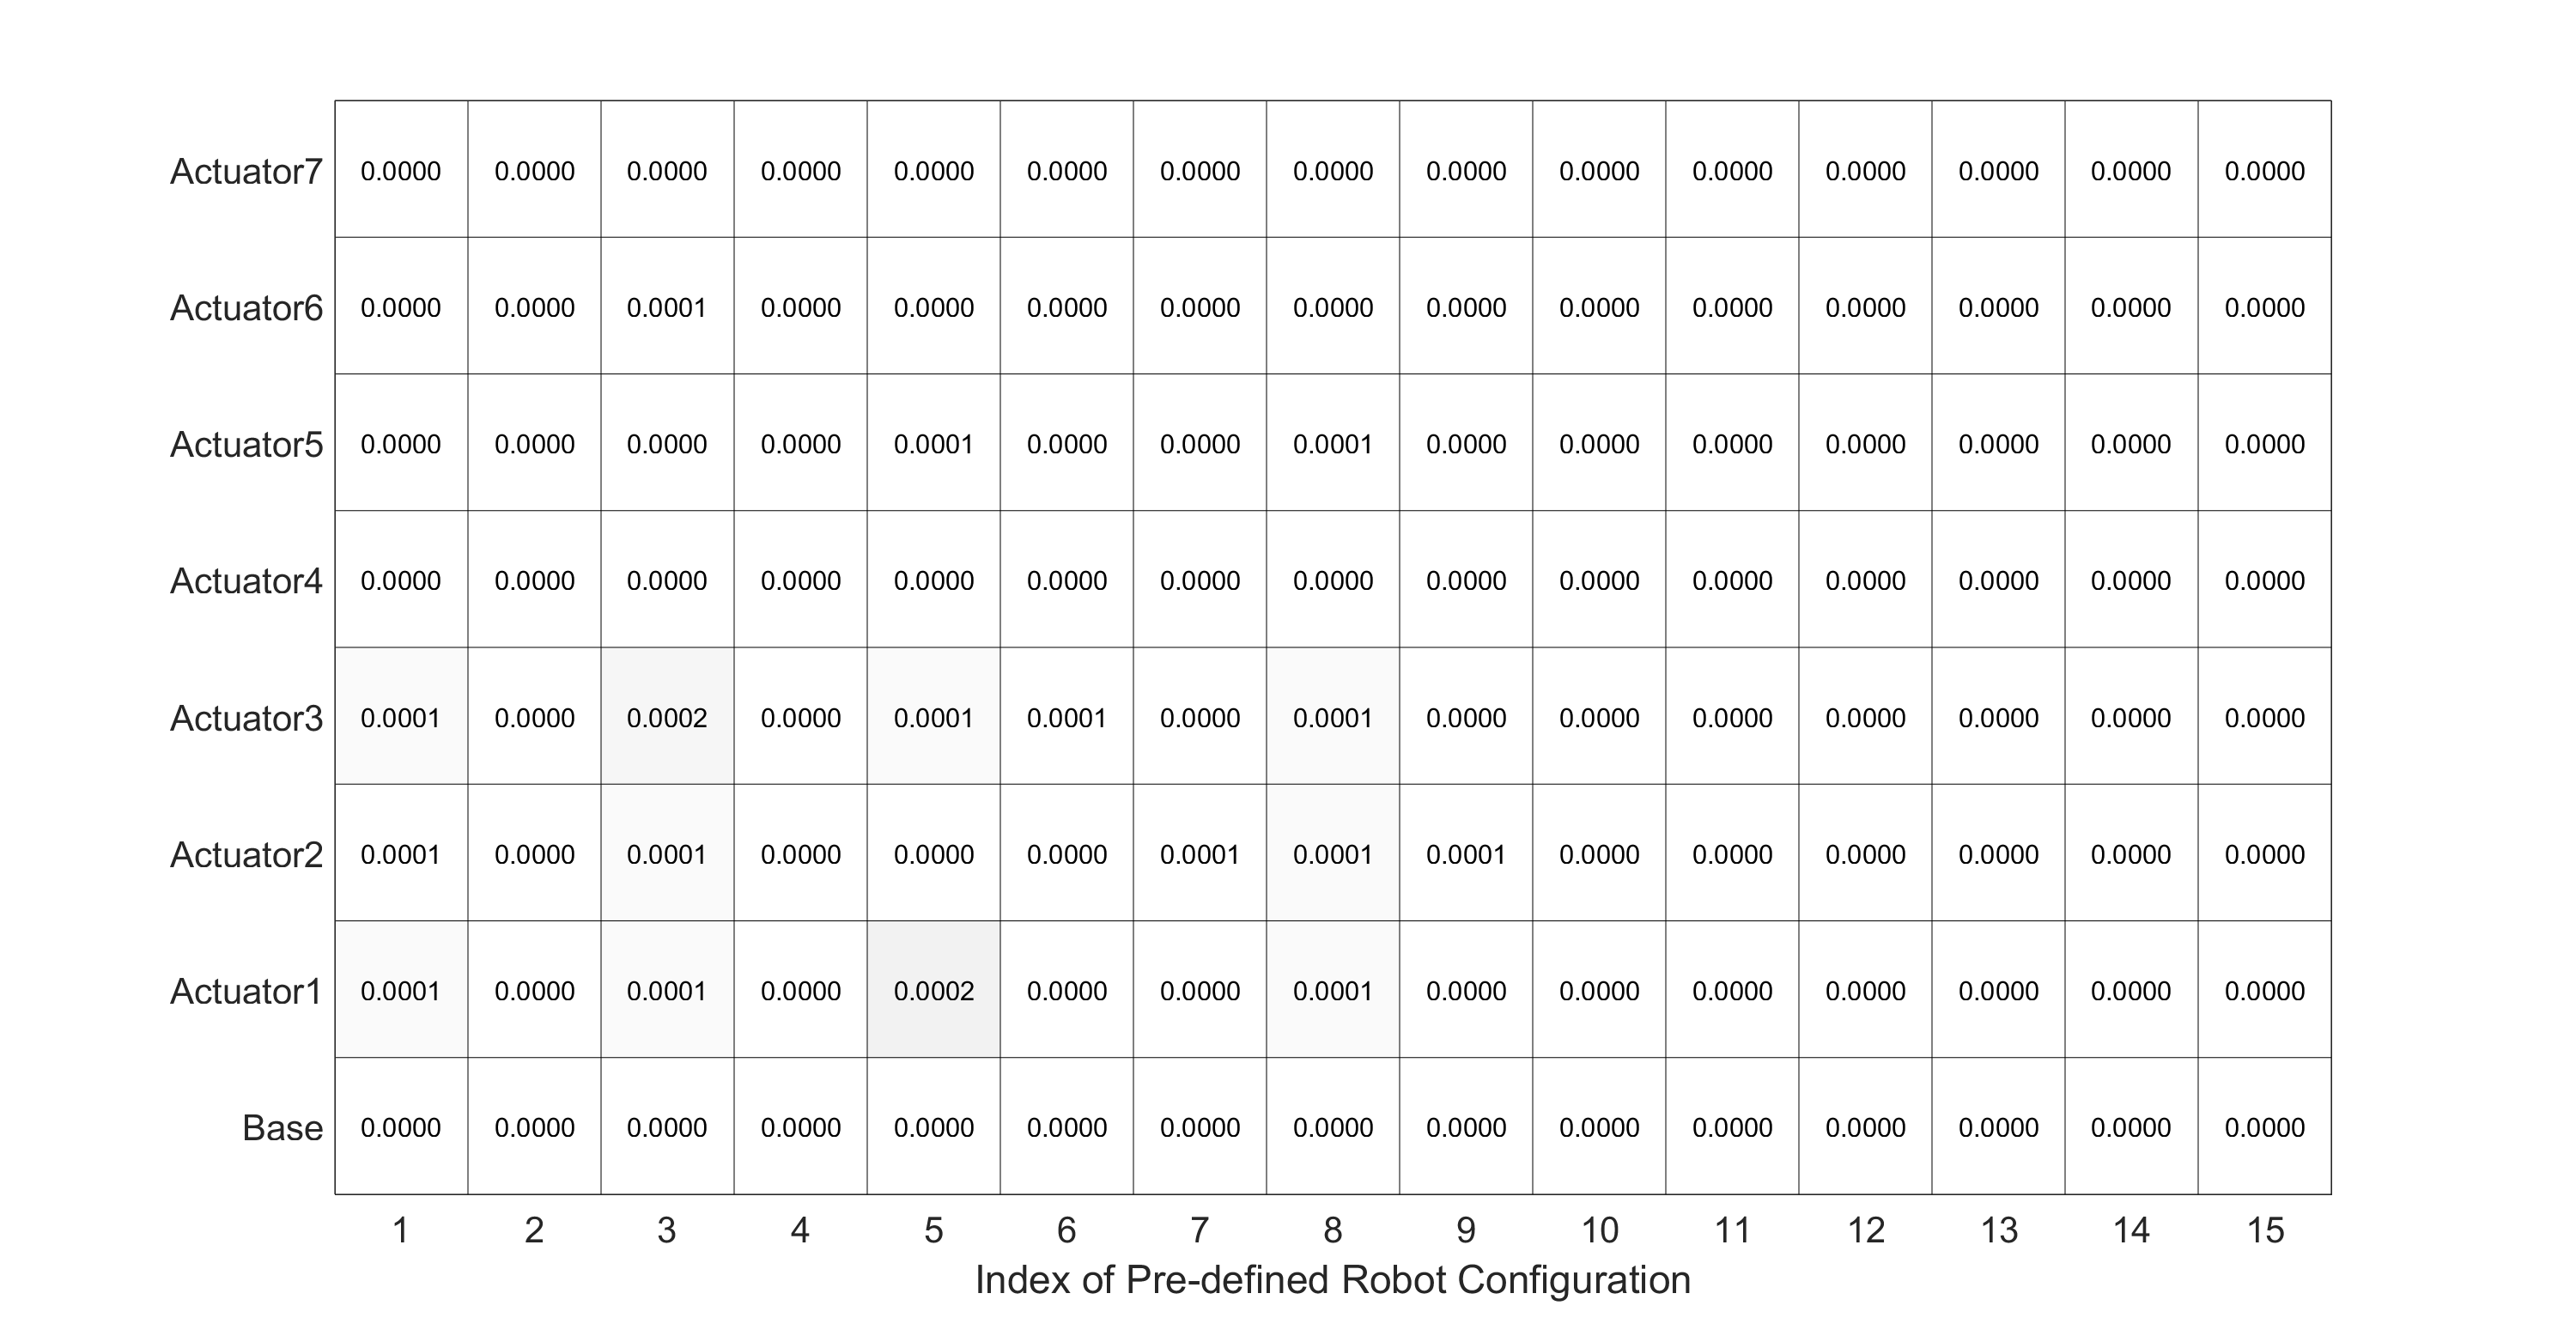
\includegraphics[width=0.9\textwidth]{./images/TorqueYErrorFB.png}%
		\caption{Error of Torque along Y axis in Nm}
		\label{fig:TorqueYErrorFB}%
	\end{center}
\end{figure}

\begin{figure}[H]
	\begin{center}
		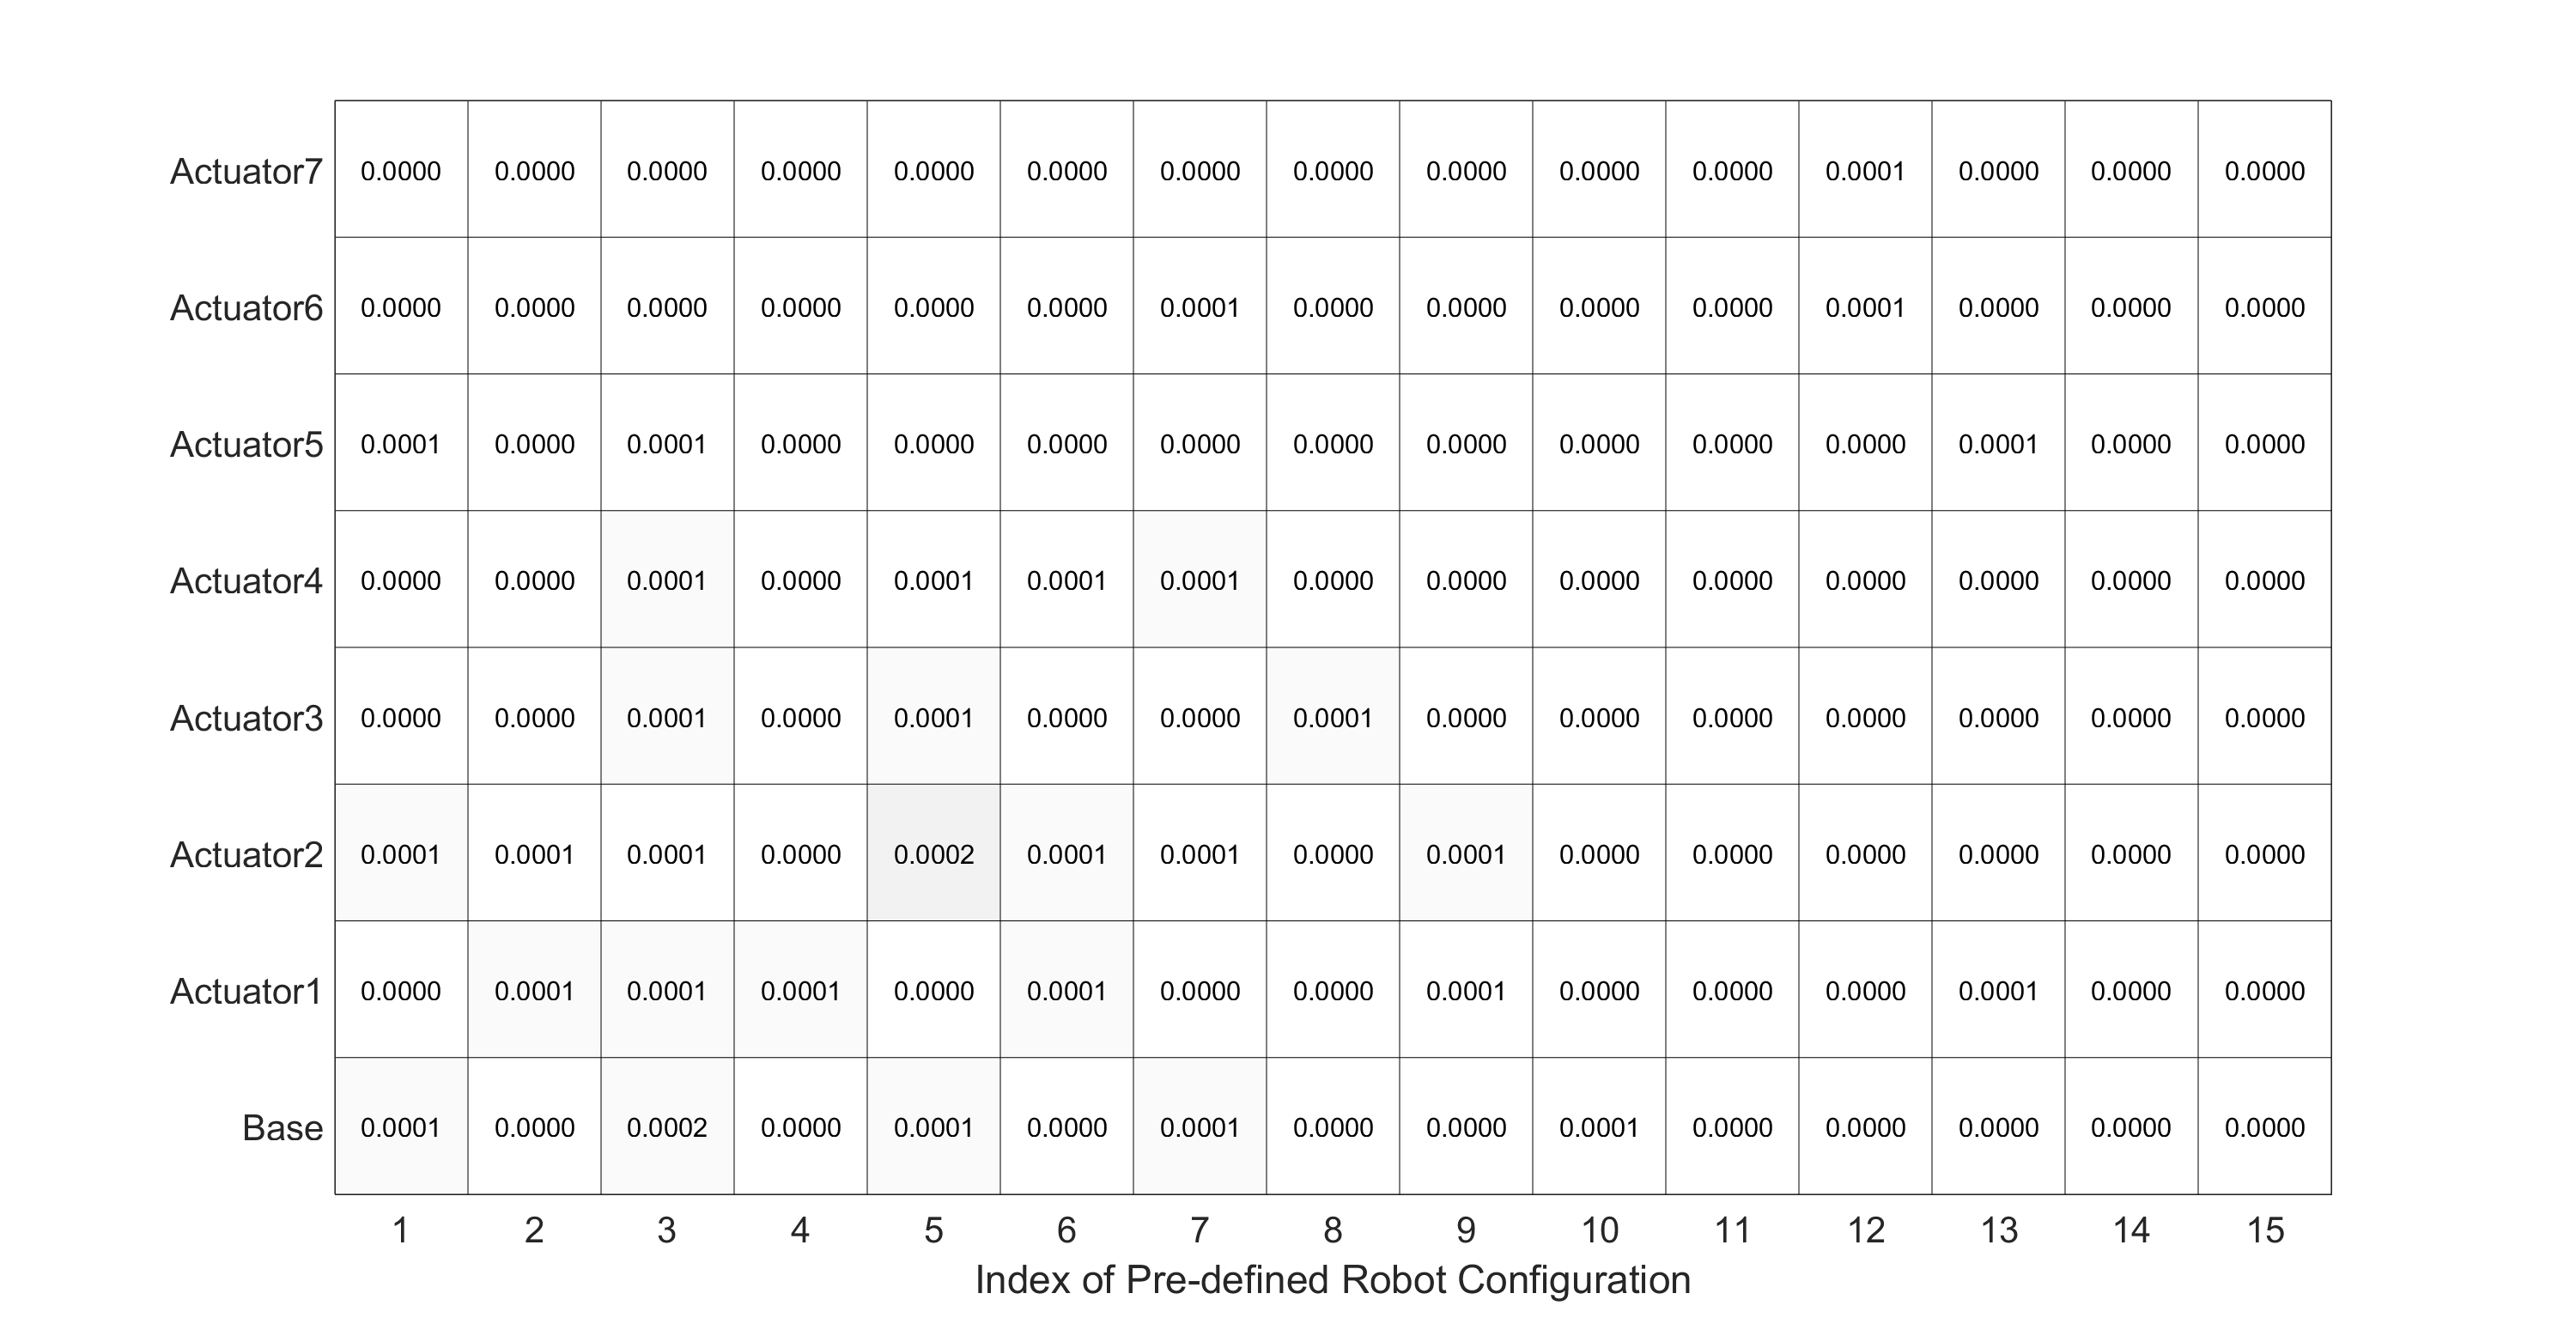
\includegraphics[width=0.9\textwidth]{./images/TorqueZErrorFB.png}%
		\caption{Error of Torque along Z axis in Nm}
		\label{fig:TorqueZErrorFB}%
	\end{center}
\end{figure}

\textbf{Therefore, we can conclude that the joint wrench data from robot base matches with the data from offline PC. The computed joint wrench in robot base performs as designed.}


The joint torque sensors are used to validate the performance of gravity model. Since joint torque sensors only measure the torque along joint axis, only the components of TorqueZ of JointWrench\_Base are used for the comparison. The differences are demonstrated in Figure \ref{fig:SensorErrortoBaseJointWrench}

\begin{figure}[H]
	\begin{center}
		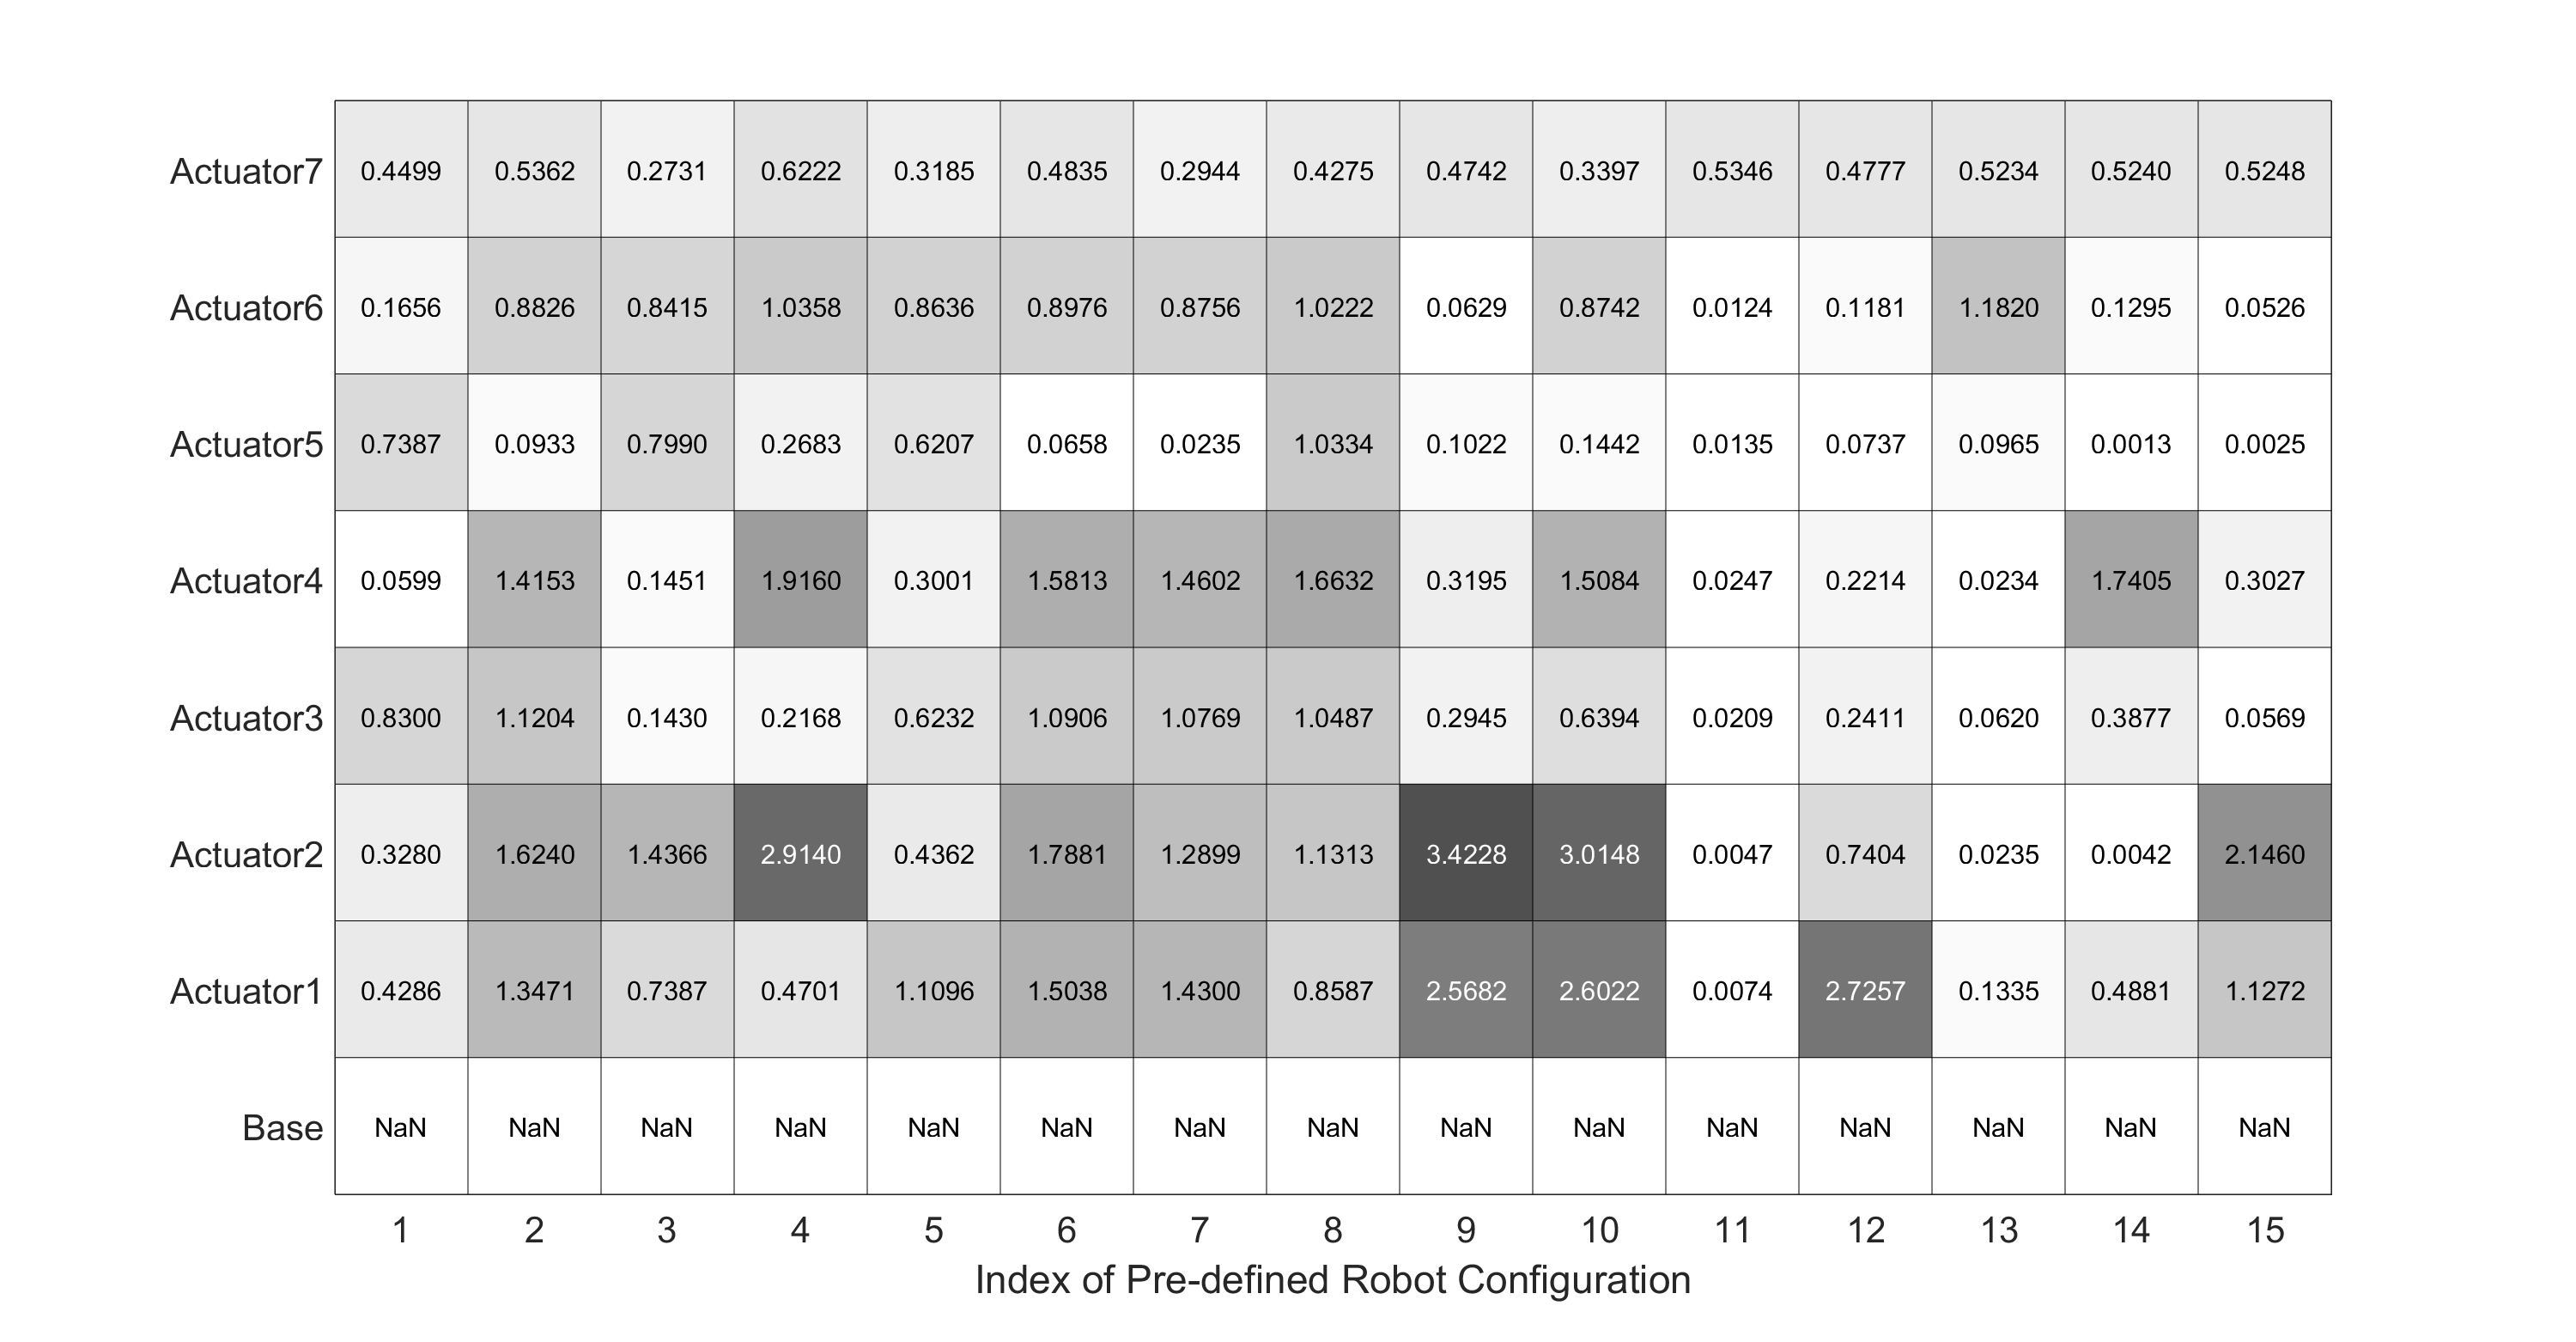
\includegraphics[width=0.9\textwidth]{./images/SensorErrortoBaseJointWrench.png}%
		\caption{Error of Torque along Z axis in Nm}
		\label{fig:SensorErrortoBaseJointWrench}%
	\end{center}
\end{figure}

The row for Base in Figure \ref{fig:SensorErrortoBaseJointWrench} is all NaN since there is no torque sensor on the robot base. The difference between joint torque sensor and  TorqueZ of JointWrench\_Base are quite evident, approximately 3.5Nm in worst cases. However, this is not enough to conclude that gravity model does not function well. The torque sensor is noisy and the seal at each joint may provide additional torque besides gravity torque. We already estimated that the seal may contribute around 2Nm to the joint. The estimation of torque sensor noise will be discussed in the Section \ref{sec:sensorReliability}.
